\documentclass[draftspec]{sbmlpkgspec}
\usepackage{tabularx}
\usepackage{tabu}
\usepackage{longtable}
\usepackage{booktabs}
\usepackage{microtype}

%macros:
\newcommand{\fixttspace}{\hspace*{1pt}}

\newcommand{\sbmlthreecore}{SBML Level~3 Core\xspace}
\newcommand{\threeone}{SBML Level~3 Version~1\xspace}
\newcommand{\threetwo}{SBML Level~3 Version~2\xspace}
\newcommand{\sbmlthreedistrib}{SBML Level~3 Package Specification for Distributions, Version~1\xspace}
\newcommand{\DistributionsPackage}{\textsf{Distributions} package\xspace}
\newcommand{\TODO}[1]{\colorbox{blue}{\textcolor{white}{TODO: #1}}}

\newcommand{\CategoricalUnivariateDistribution}{\defRef{CategoricalUnivariateDistribution}{CategoricalUnivariateDistribution-class}}
\newcommand{\Category}{\defRef{Category}{Category-class}}
\newcommand{\ContinuousUnivariateDistribution}{\defRef{ContinuousUnivariateDistribution}{ContinuousUnivariateDistribution-class}}
\newcommand{\DiscreteUnivariateDistribution}{\defRef{DiscreteUnivariateDistribution}{DiscreteUnivariateDistribution-class}}
\newcommand{\DistribInput}{\defRef{DistribInput}{DistribInput-class}}
\newcommand{\DistribBase}{\defRef{DistribBase}{DistribBase-class}}
\newcommand{\Distribution}{\defRef{Distribution}{Distribution-class}}
\newcommand{\DrawFromDistribution}{\defRef{DrawFromDistribution}{DrawFromDistribution-class}}
\newcommand{\ListOfCategories}{\defRef{ListOfCategories}{ListOfCategories-class}}
\newcommand{\ListOfDistribInputs}{\defRef{ListOfDistribInputs}{ListOfDistribInputs-class}}
\newcommand{\ListOfExternalParameters}{\defRef{ListOfExternalParameters}{ListOfExternalParameters-class}}
\newcommand{\MultivariateDistribution}{\defRef{MultivariateDistribution}{MultivariateDistribution-class}}
\newcommand{\ExternalDistribution}{\defRef{ExternalDistribution}{ExternalDistribution-class}}
\newcommand{\ExternalParameter}{\defRef{ExternalParameter}{ExternalParameter-class}}
\newcommand{\UncertBound}{\defRef{UncertBound}{UncertBound-class}}
\newcommand{\UncertStatisticSpan}{\defRef{UncertStatisticSpan}{UncertStatisticSpan-class}}
\newcommand{\UncertStatistics}{\defRef{UncertStatistics}{UncertStatistics-class}}
\newcommand{\UncertValue}{\defRef{UncertValue}{UncertValue-class}}
\newcommand{\Uncertainty}{\defRef{Uncertainty}{Uncertainty-class}}
\newcommand{\UnivariateDistribution}{\defRef{UnivariateDistribution}{UnivariateDistribution-class}}

\newcommand{\BetaDistribution}{\defRef{BetaDistribution}{BetaDistribution-class}}
\newcommand{\CauchyDistribution}{\defRef{CauchyDistribution}{CauchyDistribution-class}}
\newcommand{\ChiSquareDistribution}{\defRef{ChiSquareDistribution}{ChiSquareDistribution-class}}
\newcommand{\ExponentialDistribution}{\defRef{ExponentialDistribution}{ExponentialDistribution-class}}
\newcommand{\FDistribution}{\defRef{FDistribution}{FDistribution-class}}
\newcommand{\GammaDistribution}{\defRef{GammaDistribution}{GammaDistribution-class}}
\newcommand{\InverseGammaDistribution}{\defRef{InverseGammaDistribution}{InverseGammaDistribution-class}}
\newcommand{\LaPlaceDistribution}{\defRef{LaPlaceDistribution}{LaPlaceDistribution-class}}
\newcommand{\LogNormalDistribution}{\defRef{LogNormalDistribution}{LogNormalDistribution-class}}
\newcommand{\LogisticDistribution}{\defRef{LogisticDistribution}{LogisticDistribution-class}}
\newcommand{\NormalDistribution}{\defRef{NormalDistribution}{NormalDistribution-class}}
\newcommand{\ParetoDistribution}{\defRef{ParetoDistribution}{ParetoDistribution-class}}
\newcommand{\RayleighDistribution}{\defRef{RayleighDistribution}{RayleighDistribution-class}}
\newcommand{\StudentTDistribution}{\defRef{StudentTDistribution}{StudentTDistribution-class}}
\newcommand{\UniformDistribution}{\defRef{UniformDistribution}{UniformDistribution-class}}
\newcommand{\WeibullDistribution}{\defRef{WeibullDistribution}{WeibullDistribution-class}}
\newcommand{\BinomialDistribution}{\defRef{BinomialDistribution}{BinomialDistribution-class}}
\newcommand{\GeometricDistribution}{\defRef{GeometricDistribution}{GeometricDistribution-class}}
\newcommand{\HypergeometricDistribution}{\defRef{HypergeometricDistribution}{HypergeometricDistribution-class}}
\newcommand{\NegativeBinomialDistribution}{\defRef{NegativeBinomialDistribution}{NegativeBinomialDistribution-class}}
\newcommand{\PoissonDistribution}{\defRef{PoissonDistribution}{PoissonDistribution-class}}
\newcommand{\BernoulliDistribution}{\defRef{BernoulliDistribution}{BernoulliDistribution-class}}
\newcommand{\CategoricalDistribution}{\defRef{CategoricalDistribution}{CategoricalDistribution-class}}


\newcommand{\FluxBound}{\textbf{\class{FluxBound}}\xspace}
\newcommand{\FunctionTerm}{\textbf{\class{FunctionTerm}}\xspace}
\newcommand{\LambdaClass}{\textbf{\class{Lambda}}\xspace}
%\newcommand{\ListOf}{\textbf{\class{ListOf__}}\xspace}
\newcommand{\ChangedMath}{\textbf{\class{ChangedMath}}\xspace}
\newcommand{\Math}{\textbf{\class{Math}}\xspace}

\newcommand{\arraysshort}{arrays\xspace}
\newcommand{\arrays}{Arrays\xspace}
\newcommand{\distribshort}{\emph{distrib}\xspace}
\newcommand{\distrib}{Distributions\xspace}
\newcommand{\mathml}{MathML\xspace}
\newcommand{\uncertml}{UncertML\xspace}

\reversemarginpar  % Want "\watchout" to be put on the left, not the right.
\newcommand{\watchout}{\marginpar{\hspace*{34pt}\raisebox{-0.5ex}{\Large\ding{43}}}}
\newcommand{\controversial}{\marginpar{\hspace*{34pt}\raisebox{-0.5ex}{\Large?}}}

\begin{document}

\packageTitle{The Distributions Package\\for SBML Level 3}
\packageVersion{Version \changed{0.19} (Draft)}
\packageVersionDate{\changed{June XX, 2018}}
%\packageGeneralURL{http://sbml.org/Community/Wiki/SBML_Level_3_Proposals/Distributions_and_Ranges}
%\packageThisVersionURL{}

\author{%
  \begin{tabular}{c>{\hspace{20pt}}c}
  \multicolumn{2}{c}{\Large\bf{Authors}}\\\\ Stuart L Moodie & Lucian
  P Smith\\ \mailto{moodie@ebi.ac.uk} & \mailto{lpsmith@uw.edu}\\
  EMBL-EBI & California Institute of Technology\\ Hinxton, UK &
  Seattle, WA, USA\\ \\
  \multicolumn{2}{c}{\Large\bf{Contributors}}\\\\ Nicolas Le
  Nov\`{e}re & Darren Wilkinson\\ \mailto{lenov@babraham.ac.uk} &
  \mailto{darren.wilkinson@ncl.ac.uk}\\ Babraham Institute &
  University of Newcastle\\ Babraham, UK & Newcastle, UK\\
\\ Maciej J  Swat & Sarah Keating\\
\mailto{maciej.swat@certara.com} &  \mailto{skeating@ebi.ac.uk}
\\ QSP Simcyp & EMBL-EBI
\\ Certara, Sheffield, UK &  Hinxton, UK\\
\\
     \multicolumn{2}{c}{ Colin Gillespie}\\
     \multicolumn{2}{c}{\mailto{c.gillespie@ncl.ac.uk}}\\
     \multicolumn{2}{c}{University of Newcastle}\\
     \multicolumn{2}{c}{ Newcastle, UK}\\
\end{tabular}
}

\frontNotice{Disclaimer: This is a working draft of the SBML Level 3
  ``distib'' package proposal. It is not a normative document.  Please
  send comments and other feedback to the mailing list:
  \mailto{sbml-distrib@lists.sourceforge.net.}}

\maketitlepage
\maketableofcontents

\section*{Revision History}

\begin{edtable}{tabularx}{\linewidth}{c c c X }\toprule
\textbf{Version} & \textbf{Date} & \textbf{Author} & \textbf{Comments} \\ \midrule
0.1 (Draft) & 15 Oct 2011 & Stuart Moodie & First draft \\ \midrule
0.2 (Draft) & 16 Oct 2011 & Stuart Moodie & Added introductory text
and background info. Other minor changes etc. \\ \midrule
0.3 (Draft) & 16 Oct 2011 & Stuart Moodie & Filled empty invocation
semantics section.\\ \midrule
0.4 (Draft) & 4 Jan 2012 & Stuart Moodie & Incorporated comments from
NlN, MS and SK. Some minor revisions and corrections.\\  \midrule
0.5 (Draft) & 6 Jan 2012 & Stuart Moodie & Incorporated addition
comments on aim of package from NlN.\\ \midrule
0.6 (Draft) & 19 Jul 2012 & Stuart Moodie & Incorporated revisions
discussed and agreed at HARMONY 2012.\\ \midrule
0.7 (Draft) & 6 Aug 2012 & Stuart Moodie & Incorporated review
comments from Maciej Swat and Sarah Keating.\\ \midrule
0.8 (Draft) & 21 Dec 2012 & Stuart Moodie & Incorporated changes
suggested at combine and subsequently through list discussions.\\ \midrule
0.9 (Draft) & 9 Jan 2013 & Stuart Moodie & Incorporated corrections
and comments from Maciej Swat and Sarah Keating.\\ \midrule
0.10 (Draft) & 10 Jan 2013 & Stuart Moodie & Modified based on comments
from MS.\\ \midrule
0.11 (Draft) & 17 May 2013 & Lucian Smith & Modified based on Stuart's proposals and PWG discussion.\\ \midrule
0.12 (Draft) & June 2013 & Lucian Smith and Stuart Moodie & Modified based on HARMONY 2013 discussion.\\ \midrule
0.13 (Draft) & July 2013 & Lucian Smith and Stuart Moodie & Modified based PWG discussion, particularly with respect to UncertML.\\ \midrule
0.14 (Draft) & March 2015 & Lucian Smith  & Modified to match UncertML 3.0.\\\midrule
0.15 (Draft) & March 2015 & Lucian Smith and Sarah Keating & Modified to match UncertML 3.0 for real this time.\\ \midrule
0.16 (Draft) & March 2015 & Lucian Smith & Added information about UncertML 3.0 distributions, and the distributions custom annotations.\\\midrule
0.17 (Draft) & June 2017 & Lucian Smith & Extensive update to reflect demise of UncertML 3.0, and appearance of ProbOnto.\\\midrule
0.18 (Draft) & June 2017 & Lucian Smith & Fixes to reflect feedback on version 0.17.\\\midrule
0.19 (Draft) & June 2018 & Lucian Smith & \changed{Resolved id/name issues with SBML core l3v1 vs. l3v2.}\\
%\midrule
\bottomrule
\end{edtable}

\section{Introduction and motivation}

\subsection{What is it?}

The \distrib package (also affectionately known as \distribshort for
short) provides an extension to SBML Level 3 that enables a model to encode and sample from
both discrete and continuous probability distributions, and provide
the ability to annotate elements with information about the distribution their
values were drawn from. 
Applications of the package include for instance descriptions of
population based models: an important subset of which are
pharmacokinetic/pharmacodynamic (PK/PD) models\footnote{for more
  information see: \url{http://www.pharmpk.com/}.}, which are used to
model the action of drugs.

Note that originally the package was called Distributions and Ranges,
but Ranges are no longer in the scope, hence the name change.

\subsection{Scope}

The \distrib package adds support to SBML for sampling from a
probability distribution. In particular the following are in scope:

\begin{itemize}
\item Sampling from a continuous distribution.
\item Sampling from a discrete distribution.
\item Sampling from user-defined discrete probability density function.
\item The specification of descriptive statistics (mean, standard
  deviation, standard error, etc.).
\end{itemize}

At one point the following were considered for inclusion in this
package but are now \textbf{out of scope}:

\begin{itemize}
\item Sampling from user-defined probability density function.
\item Stochastic differential equations.
\item Other functions used to characterise a probability distribution,
  such as cumulative distribution functions (CDF) or survival functions, etc.
\end{itemize}

\subsection{This Document}

This proposal describes the consensus view of workshop participants
and subscribers to the sbml-distrib mailing list. Although it was
written by the listed authors it does not soley reflect their views nor is
it their proposal. Rather, it is their understanding of the consensus
view of what the \distrib package should do and how it should do
it. The contributors listed have made significant contributions to the
development and writing of this specification and are credited
accordingly, but a more comprehensive attribution is provided in the
acknowledgements (\sec{sec:acknowledgements}).

Finally, the authors would encourage the
reader to consider them and contribute their ideas or comments ---
indeed any feedback about this proposal --- to the \distribshort
discussion list\footnote{\mailto{sbml-distrib@lists.sourceforge.net}}.

Once the proposal is finalised this will be the first step towards the
formal adoption of the \distribshort as a package in SBML Level
3. After this, two implementations based on this proposal are required
and then the SBML editors must agree that the implementations and specification are complete. The proposal
will then provide the basis for a future package specification
document. More details of the SBML package adoption process can be
found at: \url{http://sbml.org/Documents/SBML_Development_Process}.


\subsection{Conventions used in this document}

As we are early in the package proposal process there will be some
parts of this proposal where there is no clear consensus on the
correct solution or only recent agreement or agreement by a group
which may not be representative of the SBML community as a
whole. These cases are indicated by the \controversial question mark
in the left margin (illustrated). The reader should pay particular
attention to these points and ideally provide feedback, especially if
they disagree with what is proposed. Similarly there will be points
--- especially as the proposal is consolidated --- which are agreed,
but which the reader should take note of and perhaps read again. These
points \watchout are emphasised by the hand pointer in the left margin
(illustrated).

\section{Background}

\subsection{Problems with current SBML approaches}

SBML Level 3 Core has no direct support for encoding random values
within a model. Currently there is no workaround within the core
language itself, although it is possible to define such information
using annotations within SBML itself. Frank Bergmann had proposed such
an semi-formalised extension for use with SBML L2 and L3 (See \sec{sec:annotation-scheme}).

\subsection{Past work on this problem or similar topics}

\subsubsection{The Newcastle Proposal}
\label{sec:newcastle proposal}

In 2005 there was a proposal from Colin Gillespie and others
\footnote{\url{http://sbml.org/Community/Wiki/SBML\_Leve\l_3\_Proposals/Distributions\_and\_Ranges}}
to introduce support for probability distributions in the SBML core specification. This
was based on their need to use such distributions to represent the
models they were creating as part of the BASIS project
(\url{http://www.basis.ncl.ac.uk}).

They proposed that distributions could be referred to in SBML using
the \class{csymbol} element in the \mathml subset used by
the SBML Core specification. An example is below:

\begin{example}
<xmlns=''http://www.w3.org/1998/Math/MathML''>
  <apply>
    <csymbol encoding=''text''
        definitionURL=''http://www.sbml.org/sbml/symbols/uniformRandom''>
      uniformRandom
    </csymbol>
    <ci>mu</ci>
    <ci>sigma</ci>
  </apply>
</math>
\end{example}

This required that a library of definitions be maintained as part of
the SBML standard and in their proposal they defined an initial small
set of commonly used distributions. The proposal was never
implemented.

\subsubsection{Seattle 2010}

The ``distrib'' package was discussed at the Seattle SBML Hackathon%
\footnote{\url{http://sbml.org/Events/Hackathons/The_2010_SBML-BioModels.net_Hackathon}}
and this section is an almost verbatim reproduction of Darren
Wilkinson's report on the
meeting\footnote{\url{http://sbml.org/Forums/index.php?t=tree\&goto=6141\&rid=0}}. There
Darren presented an overview of the problem%
\footnote{Slides: \url{http://sbml.org/images/3/3b/Djw-sbml-hackathon-2010-05-04.pdf}}%
\footnote{Audio: \url{http://sbml.org/images/6/67/Wilkinson-distributions-2010-05-04.mov}},
building on the old proposal from the Newcastle group (see above:
\ref{sec:newcastle proposal}).  There was broad support at the meeting
for development of such a package, and for the proposed feature
set. Discussion following the presentation led to a consensus on the
following points:

\begin{itemize}
\item There is an urgent need for such a package.
\item It is important to make a distinction between a description of
  uncertainty regarding a model parameter and the mechanistic process
  of selecting a random number from a probability distribution, for
  applications such as parameter scans and experimental design
\item It is probably worth including the definition of PMFs, PDFs and CDFs in the package
\item It is worth including the definition of random distributions using particle representations within such a package, though some work
 still needs to be done on the precise representation
\item It could be worth exploring the use of xinclude to point at particle
representations held in a separate file
\item Random numbers must not be used in rate laws or anywhere else that
 is continuously evaluated, as then simulation behaviour is not
 defined
\item Although there is a need for a package for describing extrinsic
 noise via stochastic differential equations in SBML, such mechanisms
 should not be included in this package due to the considerable
 implications for simulator developers
\item We probably don't want to layer on top of \uncertml
 (www.uncertml.org), as this spec is fairly heavy-weight, and
 somewhat tangential to our requirements
\item A random number seed is not part of a model and should not be
 included in the package
\item The definition of truncated distributions and the specification of
 hard upper and lower bounds on random quantities should be
 considered.
\end{itemize}

It was suggested that new constructs should be introduced into SBML by
the package embedded as user-defined functions using the following
syntax:

\begin{example}
<listOfFunctionDefinitions>
  <functionDefinition id="myNormRand">
    <distrib:####>
      #### distrib binding information here ####
    </distrib:####>
    <math>
      <lambda>
        <bvar>
          <ci>mu</ci>
          <ci>sigma</ci>
        </bvar>
        <ci>mu</ci>
      </lambda>
    </math>
  </functionDefinition>
</listOfFunctionDefinitions>
\end{example}

which allows the use of a "default value" by simulators which do not
understand the package (but simulators which do will ignore the <math>
element). The package would nevertheless be "required", as it will not
be simulated correctly by software which does not understand the
package.

Informal discussions following the break-out covered topics such as:

\begin{itemize}
\item how to work with vector random quantities in the absence of the vector
element in the MathML subset used by SBML
\item how care must be taken with the semantics of random variables
  and the need to both:
\begin{itemize}
\item reference multiple independent random quantities at a given
  time
\item make multiple references to the same random quantity at a given
time.
\end{itemize}
\end{itemize}

\subsubsection{Hinxton 2011}

Detailed discussion was continued at the Statistical Models Workshop
in Hinxton in June 2011%
\footnote{\url{http://sbml.org/Events/Other_Events/statistical_models_workshop_2011}}. There
those interested in representing Statistical Models in SBML came
together to work out the details of how this package would work in
detail. Dan Cornford from the \uncertml
project\footnote{\url{http://www.uncertml.org/}} attended the meeting
and described how that resource could be used to describe uncertainty
and in particular probability distributions. Perhaps the most
significant decision at this meeting was to adopt the \uncertml
resource as a controlled vocabulary that is referenced by the \distrib package.

Much has changed since this meeting, but the output from this meeting
was the basis for the first version of this proposal.


\subsubsection{HARMONY 2012: Maastricht}

Two sessions were dedicated to discussion of \distrib at HARMONY based
around the proposals described in version 0.5 of this document. In
addition there was discussion about the \arrays proposal which was
very helpful in solving the problem of multivariate distributions in
\distrib. The following were the agreed outcomes of the meeting:

\begin{itemize}
\item The original proposal included UncertML markup directly in the
  function definition. This proved unwieldy and confusing and has been
  replaced by a more elegant solution that eliminates the UncertML
  markup and integrates well with the fallback function (see details
  below).
\item Multivariate distributions can be supported using the \arrays
  package to define a covariance matrix.
\item User defined continuous distributions would define a PDF in
  \mathml.
\item Usage semantics were clarified so that invokation of a function
  definition implied a value was sampled from the specified
  distribution.
\item It was agreed from which sections of an SBML model a
  distribution could be invoked.
\item Statistical descriptors of variables (for
  example mean and standard deviation) would be separated from
  \distrib and either provided in a new package or in a later version
  of SBML L3 core.
\end{itemize}

\subsubsection{COMBINE 2012: Toronto}

The August proposal was reviewed and an improvement was agreed to
the user-defined PMF part of the proposal. In particular is was agreed
that the categories should be defined by \distribshort classes rather
than by passing in the information as an array. Questions were also raised
about whether \uncertml was suitably well defined to be used as an
external definition for probability distributions. This was resolved
subsequent to the meeting with a teleconference to Dan Cornford and
colleagues. These changes are incorporated here. Finally, there was
considerable debate about whether to keep the dependence of
\distribshort on the Arrays package in order to support multi-variate
distributions. The outcome was an agreement that we would review this
at the end of 2012, based on the results of an investigation
into how feasible it would be to implement \arrays as a package.

\subsubsection{2013 Package Working Group discussions}

Early 2013 saw a good amount of discussion on the \distribshort Package Working Group mailing list, spurred by proposals by Stuart Moodie\footnote{\url{http://thestupott.wordpress.com/2013/03/12/an-improved-distrib-proposal/}}.  While not all of his suggestions ended up being fully accepted by the group, several changes were accepted, including:

\begin{itemize}
\item To use UncertML as actual XML, instead of as a set of reference definitions.
\item To use UncertML to encode descriptive statistics of SBML elements such as mean, standard deviation, standard error, etc.) bringing this capability back in scope for this package.
\end{itemize}


\subsubsection{HARMONY 2013: Connecticut}

At HARMONY at UConn in Connecticut, further discussions revealed the importance of distinguishing the ability to describe an element as a distributed variable vs. a function call within the model performing a draw from a distribution.

We also decided to discard the encoding of explicit PDFs for now, as
support for it is remarkably complicated, and there no demand for
it. The current design could be extended to support this feature so if
there is demand for it in the future support for explicit PDFs could
be reintroduced.

\subsubsection{Early 2017 and HARMONY: Seattle}

In early 2017, it became clear that UncertML was no longer being worked on; the web page had lapsed, and its authors had moved on to other things.  At the same time, the ProbOnto ontology (\citealt{swat:2016}; \url{http://probonto.org/}) was developed that included all the distributions from UncertML as well as a huge number of other distributions.  On the mailing list, it was discussed whether to create essentially our own version of UncertML, or to implement a generic 'reference' format that used ProbOnto.  The v0.17 draft specification was developed as a compromise 'hybrid' system that did parts of both, so that basic distributions would be hard-coded, but the ability to reference any ProbOnto ontology would also be present.  The hope is that with working examples of both approaches, either the hybrid approach will be approved, or if one is preferred, the other approach may be removed.  This version of the specification was created for presentation at HARMONY 2017 in Seattle.


\section{Proposed syntax and semantics}

\subsection{Overview}

Following the precedent set by the SBML Level~3 Core specification
document, we use UML~1.0 (Unified Modeling Language;
\citealt{eriksson:1998,oestereich:1999}) class diagram notation to
define the constructs provided by this package.  We also use color in
the diagrams to carry additional information for the benefit of those
viewing the document on media that can display color.  The following are
the colors we use and what they represent:

\begin{itemize}

\item[\raisebox{2.75pt}{\colorbox{black}{\rule{0.8pt}{0.8pt}}}]
  \emph{Black}: Items colored black in the UML diagrams are components
  taken unchanged from their definition in the SBML Level~3 Core
  specification document.

\item[\raisebox{2.75pt}{\colorbox{mediumgreen}{\rule{0.8pt}{0.8pt}}}]
  \emph{\textcolor{mediumgreen}{Green}}: Items colored green are
  components that exist in SBML Level~3 Core, but are extended by this
  package.  Class boxes are also drawn with dashed lines to further
  distinguish them.

\item[\raisebox{2.75pt}{\colorbox{darkblue}{\rule{0.8pt}{0.8pt}}}]
  \emph{\textcolor{darkblue}{Blue}}: Items colored blue are new
  components introduced in this package specification.  They have no
  equivalent in the SBML Level~3 Core specification.

\item[\raisebox{2.75pt}{\colorbox{red}{\rule{0.8pt}{0.8pt}}}]
  \emph{\textcolor{red}{Red lines}}: Classes with red lines in the corner are fully defined in a different figure.

\end{itemize}

We also use the following typographical conventions to distinguish the
names of objects and data types from other entities; these conventions
are identical to the conventions used in the SBML Level~3 Core specification
document:

\begin{description}
  
\item \abstractclass{AbstractClass}: Abstract classes are never
  instantiated directly, but rather serve as parents of other classes.
  Their names begin with a capital letter and they are printed in a
  slanted, bold, sans-serif typeface.  In electronic document formats,
  the class names defined within this document are also hyperlinked to
  their definitions; clicking on these items will, given appropriate
  software, switch the view to the section in this document containing
  the definition of that class.  (However, for classes that are
  unchanged from their definitions in SBML Level~3 Core, the class names
  are not hyperlinked because they are not defined within this
  document.)
  
\item \class{Class}: Names of ordinary (concrete) classes begin with a
  capital letter and are printed in an upright, bold, sans-serif
  typeface.  In electronic document formats, the class names are also
  hyperlinked to their definitions in this specification document.
  (However, as in the previous case, class names are not hyperlinked if
  they are for classes that are unchanged from their definitions in the
  SBML Level~3 Core specification.)

\item \token{SomeThing}, \token{otherThing}: Attributes of classes, data
  type names, literal XML, and tokens \emph{other} than SBML class
  names, are printed in an upright typewriter typeface.  Primitive types
  defined by SBML begin with a capital letter; SBML also makes use of
  primitive types defined by XML
  Schema~1.0~\citep{biron:2000,fallside:2000,thompson:2000}, but
  unfortunately, XML~Schema does not follow any capitalization
  convention and primitive types drawn from the XML~Schema language may
  or may not start with a capital letter.

\item \token{[elementName]}:  In some cases, an element may contain a child of any class inheriting from an abstract base class.  In this case, the name of the element is indicated by giving the abstract base class name in brackets, meaning that the actual name of the element depends on whichever subclass is used, with capitalization following the capitalization of the name in brackets.

\end{description}

For other matters involving the use of UML and XML, we follow the
conventions used in the SBML Level~3 Core specification document.  


\subsection{Namespace URI and other declarations necessary for using this package}
\label{xml-namespace}

Every SBML Level~3 package is identified uniquely by an XML namespace URI.  For an SBML document to be able to use a given Level~3 package, it must declare the use of that package by referencing its URI.  \changed{This version of the \distrib package has two URIs, depending on which version of core SBML is being used:}
\begin{blockChanged}
\begin{center}
\uri{http://www.sbml.org/sbml/level3/version1/distrib/version1}
\end{center}
\begin{center}
\uri{http://www.sbml.org/sbml/level3/version2/distrib/version1}
\end{center}
\end{blockChanged}


Note that the \distrib package may be used with both \threeone and \threetwo documents, \changed{with the only semantic change between the two present in the \DistribBase class. Note that if used with \threeone the corresponding \distrib namespace for \threeone must be used and similarly if \threetwo is being used, the \distrib namespace must be the one for \threetwo.}


In addition, SBML documents using a given package must indicate whether the package may be used to change the mathematical meaning of \sbmlthreecore elements.  This is done using the attribute \token{required} on the \token{<sbml>} element in the SBML document.  For the \distrib package, the value of this attribute must be \val{true}, as the \DrawFromDistribution element overrides the core definition of a \FunctionDefinition.  Note that the value of this attribute must \emph{always} be set to \val{true}, even if the particular model does not contain any \DrawFromDistribution elements.

The following fragment illustrates the beginning of a typical SBML model using \threeone and this version of the \distrib package:

\begin{example}
<?xml version="1.0" encoding="UTF-8"?>
<sbml xmlns="http://www.sbml.org/sbml/level3/version1/core" level="3" version="1"
      xmlns:distrib="http://www.sbml.org/sbml/level3/version1/distrib/version1"
      distrib:required="true">
\end{example}


The following fragment illustrates the beginning of a typical SBML model using \threetwo and this version of the \distrib package:

\begin{example}
<?xml version="1.0" encoding="UTF-8"?>
<sbml xmlns="http://www.sbml.org/sbml/level3/version2/core" level="3" version="2"
      xmlns:distrib="http://www.sbml.org/sbml/level3/version2/distrib/version1"
      distrib:required="true">
\end{example}

\subsection{Primitive data types}
\label{new-primitive-types}

The \distrib package uses data types described in Section~3.1 of the \sbmlthreecore specification, and adds the additional primitive types described below.

\subsubsection{Type \fixttspace\primtypeNC{ExternalRef}}
\label{sec:primtype-externalref}

The type \primtype{ExternalRef} is derived from \primtype{string} with the additional requirement that it be a valid URI.  An \primtype{ExternalRef} is used in \distrib to point to ontologies such as ProbOnto~\citep{swat:2016} which contain defined distributions and parameters. 


\subsubsection{Type \fixttspace\primtypeNC{UncertId}}
\label{sec:primtype-uncertid}

The type \primtype{UncertId} is derived from \primtype{SId} (\sbmlthreecore specification Section~3.1.7) and has identical syntax.  The \primtype{UncertId} type is used to create local ids that can be used in the extended \FunctionDefinition objects to refer to the arguments of the function, in much the same way that the identities of the \token{bvar} elements are used in MathML \token{lambda} elements.  Each \primtype{UncertId} has a scope local to the \DrawFromDistribution in which it is found.  The
equality of \primtype{UncertId} values is determined by an exact
character sequence match; i.e., comparisons of these identifiers must be
performed in a case-sensitive manner.


\subsubsection{Type \fixttspace\primtypeNC{UncertIdRef}}
\label{sec:primtype-uncertidref}

Type \primtype{UncertIdRef} is used to reference different elements in different contexts.  Inside a \FunctionDefinition, an \primtype{UncertIdRef} may only reference an \primtype{UncertId} from a \DistribInput from that same \FunctionDefinition.  Outside a \FunctionDefinition, an \primtype{UncertIdRef} may reference any element with an \primtype{SId} that has mathematical meaning: even elements from other packages, and not in \sbmlthreecore.  In the context of an \threeone document, this still holds true.  Even though \threeone elements with \primtype{SIdRef} attributes cannot reference package elements, this does not preclude \distrib elements from doing so.

If a referenced \primtype{SId} is from a package that is not understood by the software reading the model, the meaning of the \primtype{UncertIdRef} is undefined.   If an interpreter does not understand an id and cannot tell whether that id came from a not-understood package, it may issue a warning.


As with \primtype{UncertId}, the equality of
\primtype{UncertIdRef} values is determined by exact character sequence
match; i.e., comparisons of these identifiers must be performed in a
case-sensitive manner.



\subsection{Defining Distributions}

\subsubsection{The approach}

The \distrib package has two very simple purposes. First, it provides a
mechanism for sampling a random value from a probability
distribution. This implies that it must define the probability distribution and then must sample a
random value from that distribution.

Secondly, it provides a mechanism for describing elements with information about their uncertainty.  One common use case for this will be to provide the standard deviation for a value.  Another may be describing a parameter's distribution, so that a better search can be performed in a parameter scan experiment.

These purposes are achieved by extending \FunctionDefinition and \SBase, which in turn use the \Distribution and \UncertStatistics classes, modeled after \uncertml.  Several distributions and statistics are defined explicitly in this specification, but more can be defined by referencing the external ontology such as the ProbOnto ontology through the \ExternalDistribution and \ExternalParameter classes.

It is hoped that with this approach, modelers may use the \Distribution classes defined in this specification with a reasonable expectation of various software packages recognizing and replicating those distributions.  However, if another distribution is required, those distributions may still be encoded, even if this makes the model less exchangeable.

When a distribution is defined in a \FunctionDefinition, it is sampled when it is invoked. To reuse a sampled value, the value must be assigned to a parameter first, such as through the use of an \InitialAssignment or \EventAssignment.  When a distribution is defined elsewhere, that information may be used outside of the model, using whatever methodology is appropriate to answer the question being pursued.


\begin{blockChanged}
\subsection{The \DistribBase class}
\label{sec:DistribBase-class}
\label{DistribBase-class}
\label{sec:idname}

The \DistribBase class is an abstract base class which is the parent class for every class in this \distrib package.  Its sole purpose is to encapsulate how this package handles the fact that in \threetwo, the attributes \token{id} and \token{name} were added to \SBase.  It defines attributes 'distrib:id' and 'distrib:name' as optional, so that they can be used in \threeone documents where those attributes would otherwise not exist.  However, in \threetwo documents, 'distrib:id' and 'distrib:name' may not be used: the core attributes \token{id} and \token{name} should be used instead.  In this way, every \distrib element will always have exactly one id and exactly one name.

The meaning of these attributes is identical, regardless of the level/version of the document in which they appear.  When a subclass makes one of the attributes required (as the \token{id} of the \DistribInput class), this means that it must have the 'distrib:id' attribute in a \threeone document, or an \token{id} attribute in a \threetwo document.
\end{blockChanged}

The \token{id} attribute is of type \primtype{SId}, and must be unique among other ids in the \primtype{SId} namespace in the parent \Model, and has no mathematical meaning, unless stated otherwise in the definition of that object.  The \token{name} attribute is of type \primtype{string}, and is provided to allow the user to define a human-readable label for the object, and has no uniqueness restrictions.

\begin{figure}[bh]
  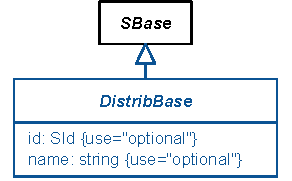
\includegraphics{figs/distribBase.pdf}
  \caption{\changed{The definition of the \DistribBase class.  The \token{id} and \token{name} attributes defined are optional, but must not be used in \threetwo documents.}}
  \label{fig:distribBase}
\end{figure}

\subsection{The extended \class{FunctionDefinition} class}
\label{extended-functiondefinition-class}

To model random processes, this package extends the \FunctionDefinition class as
can be seen in the UML representation in \fig{fig:funcdef}. The redefined \FunctionDefinition optionally
contains a single \token{drawFromDistribution} child.

The \FunctionDefinition class may or may not still contain the \mathml block containing the standard SBML function definition if used in an \threetwo document, but it must contain this MathML block if used in an \threeone document, because that element is required in that level and version.  If present, the MathML should be ignored, but may ensure a degree of backwards compatibility for SBML readers and validators that do not understand the \distribshort package.

\begin{figure}[htb]
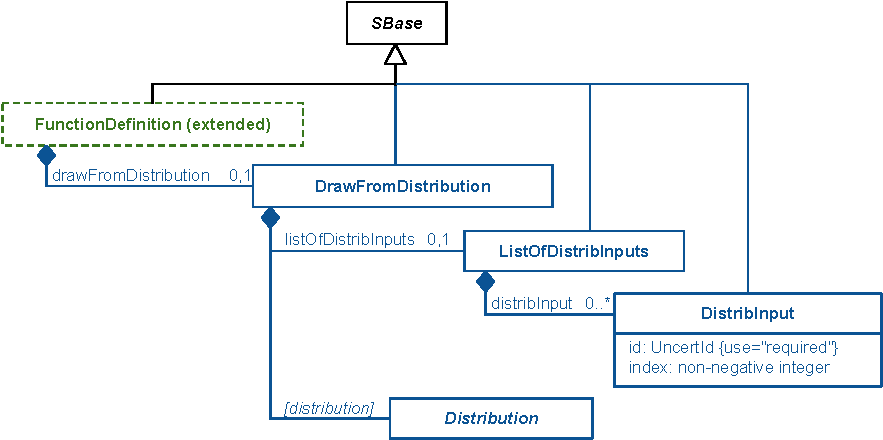
\includegraphics[width=0.75\linewidth]{figs/extended-functionDefinition.pdf}
\caption{The definition of the extended \FunctionDefinition class, plus the \DrawFromDistribution, \ListOfDistribInputs, and \DistribInput classes.  The \Distribution class is used here, but defined later.  A \DrawFromDistribution element must have exactly one \Distribution child.  Together, these classes provide a way to transform a \FunctionDefinition to sample from a distribution.}
\label{fig:funcdef}
\end{figure}


As outlined above, the \FunctionDefinition class is extended to contain a \DrawFromDistribution child, which overrides \changed{the <lambda> element of the \Math child} present in the \FunctionDefinition.  Software that does not support \distribshort could potentially invoke the original \Math of the \FunctionDefinition (see \ref{sec:fallbackfunc}) instead.



In the \Model, an extended \FunctionDefinition may be used in any \mathml elsewhere in the document to perform a draw from a distribution.  This draw will be unique for every use of the \FunctionDefinition, whether or not the draw is performed at the same simulation time as a different draw (for example, if used in two different \InitialAssignment elements).



\subsection{The \class{DrawFromDistribution} class}
\label{DrawFromDistribution-class}
\label{drawfromdistribution-class}

As illustrated in \fig{fig:funcdef}, the \DrawFromDistribution class may have a \ListOfDistribInputs child, which may in turn contain any number of \DistribInput children, which act as the arguments to the function--they serve the same role as the \token{bvar} elements of the \LambdaClass child of a \FunctionDefinition.  The order of arguments is determined by the \token{index} attribute:  the first argument (if any) must have an index of \val{0}, the second of \val{1}, etc.  If no \ListOfDistribInputs is provided, or if one is provided with no \DistribInput children, the function contains no arguments.

The \DrawFromDistribution must also have a \Distribution child, representing the distribution from which to draw a value.  Because \Distribution is an abstract class, the name of the element will be the name of the class of the particular distribution being used, with its first letter made lower case (so, \val{normalDistribution} for \NormalDistribution, \val{studentTDistribution} for \StudentTDistribution, etc.).  Within this \Distribution, any \primtype{UncertIdRef} must reference the \primtype{UncertId} of a \DistribInput for the \FunctionDefinition in which it appears.

\subsubsection{Attributes inherited from \SBase}

A \DrawFromDistribution always inherits the optional \token{metaid} and \token{sboTerm} attributes, and inherits optional \token{id} and \token{name} attributes as described in \sec{sec:idname}.  The \token{id} of a \DrawFromDistribution has no mathematical meaning.


\subsection{The \class{ListOfDistribInputs} class}
\label{ListOfDistribInputs-class}
\label{listofdistribinputs-class}

The \ListOfDistribInputs class, like other \ListOf classes in \sbmlthreecore, is a container for zero or more \DistribInput objects.  If empty, it simply means that no child \DistribInput objects are defined for its parent, and is equivalent to not including the \ListOfDistribInputs object at all.  This situation defines an extended \FunctionDefinition with zero arguments, and might be useful if the list is annotated with the reason why it is empty, for example.


\subsection{The \class{DistribInput} class}
\label{DistribInput-class}
\label{distribinput-class}

The \DistribInput class mimics the \token{bvar} elements of MathML lambda functions.  It must have an \token{id} attribute of type \primtype{UncertId} and an \token{index} attribute of type \primtype{non-negative integer}.

Each \DistribInput element represents an argument to the function, and serves as a local identifier, referenced only by the \Distribution class. See the examples in \ref{sec:fd-examples} for more details.

If the \LambdaClass child of the \FunctionDefinition is present, it must have the same number of \token{bvar} children as the \DrawFromDistribution has \DistribInput children.  They do not, however, have to have the same ids:  the \token{bvar} ids are defined as being local to the \LambdaClass function in much the same way that the \DistribInput ids are defined as being local to the \DrawFromDistribution object.

Each \token{index} attribute on a \DistribInput within a \ListOfDistribInputs element must have a unique value, numbered consecutively from \val{0}:  if one \DistribInput is present, its \token{index} value must be \val{0}; if there are two, they must have \token{index} values of \val{0} and \val{1}, etc. \changed{Where the \FunctionDefinition also contains a \Math child the values of the \token{index} relates the \DistribInput to the the <bvar> element in the corresponding position.}

\subsubsection{Attributes inherited from \SBase}

A \DistribInput always inherits the optional \token{metaid} and \token{sboTerm} attributes, and inherits the \token{id} and \token{name} attributes as described in \sec{sec:idname}.  The \token{id} of a \DistribInput has no external mathematical meaning, is required, and is of type \primtype{UncertId}, as described above.  Note that in an \threetwo document, a \DistribInput must either have an \token{id} in the core namespace, or an \token{id} in the \distrib namespace (but not both).

\begin{figure}[htb]
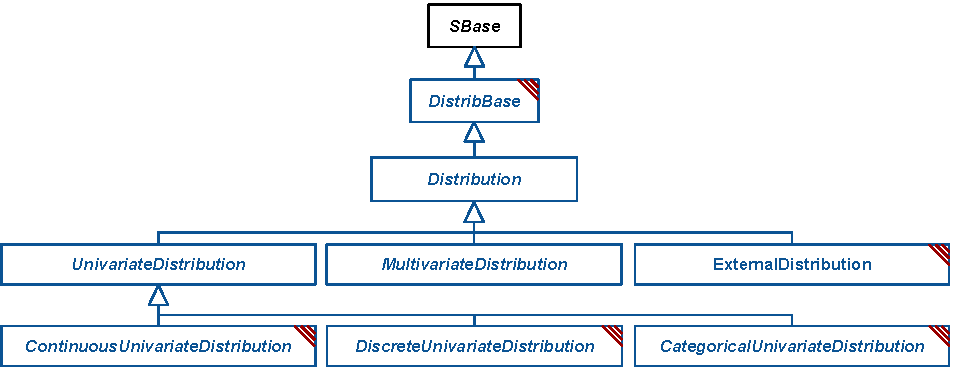
\includegraphics[width=0.75\linewidth]{figs/distribution.pdf}
\caption{The definition of the abstract \Distribution class, plus the abstract \UnivariateDistribution and \MultivariateDistribution classes.  Also shown are the \ContinuousUnivariateDistribution, \DiscreteUnivariateDistribution, \CategoricalUnivariateDistribution, and \ExternalDistribution classes, defined later.  Note that the \MultivariateDistribution class is only defined here, and, as such, has no concrete classes that derive from it at this time in this version of the \distrib specification.  If further discussion reveals a need for them, it is shown here as an example of where it would be defined, but may disappear from a future version of the spec if no derived class for it is ever defined.}
\label{fig:distribution}
\end{figure}

\subsection{The \class{Distribution} class}
\label{Distribution-class}
\label{distribution-class}

The \Distribution class is the abstract class from which all \distrib distributions are derived.  They are organized here in much the same way they were in \uncertml, by whether they are univariate or multivariate, and whether they are continuous, discrete, or categorical.  In addition, the \ExternalDistribution inherits from \Distribution, as a 'generic' distribution definition class that allows the user to define any distribution in an external ontology such as ProbOnto.

When a \Distribution is encountered, its parent \FunctionDefinition is defined as sampling from the defined distribution, and returning that sample.  It may contain any number of \token{UncertIdRef} strings, each of which must correspond to an \token{UncertId} defined in a \DistribInput in the same function.

{\color{red} Lucian: \controversial NOTE!  There are too many distributions defined in this version of the \distrib specification!  This is done on purpose.  The goal of this draft of the specification is not to be normative, but to lay out the details of everything that might possibly be wanted, with the intent of reducing the number to what is actually going to be used and implemented in a subsequent draft, based on user and developer feedback.  As a start, then, every single univariate distribution defined in \uncertml, plus the \RayleighDistribution (defined in Frank's annotation scheme), is presented.  The idea is that developers first implement what is useful for them, then we trim the list to only what at least one developer implemented, then we give developers the newly-winnowed list and say 'this is what other people want' and ask them to fill in the gaps.  It is predicted that the final number of pre-defined distributions will number about a dozen or so.}

In this draft of the \distrib specification, no mixed distributions and no multivariate distributions are presented, as the author has not seen any call for these distributions specifically, and believes that the generic \ExternalDistribution distribution could cover those cases on an as-needed basis.  If this turns out to not be the case, those distributions will be added to a subsequent version of this specification.  The use of the Arrays package would be required for any multivariate distribution.

\subsubsection{Attributes inherited from \SBase}

A \Distribution always inherits the optional \token{metaid} and \token{sboTerm} attributes, and inherits optional \token{id} and \token{name} attributes as described in \sec{sec:idname}.  The \token{id} of a \Distribution has no mathematical meaning.


\subsection{The \class{UnivariateDistribution} class}
\label{UnivariateDistribution-class}
\label{univariatedistribution-class}

The \UnivariateDistribution class is an abstract class that derives from the \Distribution abstract class, and which has three derived classes itself: \ContinuousUnivariateDistribution, \DiscreteUnivariateDistribution, and \CategoricalUnivariateDistribution.  It is provided as a bookkeeping class to distinguish it from other types of distributions.


\subsection{The \class{MultivariateDistribution} class}
\label{MultivariateDistribution-class}
\label{multivariatedistribution-class}

The \MultivariateDistribution class is an abstract class with no derived classes in the current specification, but some could be added in the future.  Most likely, it will be removed from the final version of the spec.


\begin{figure}[htb]
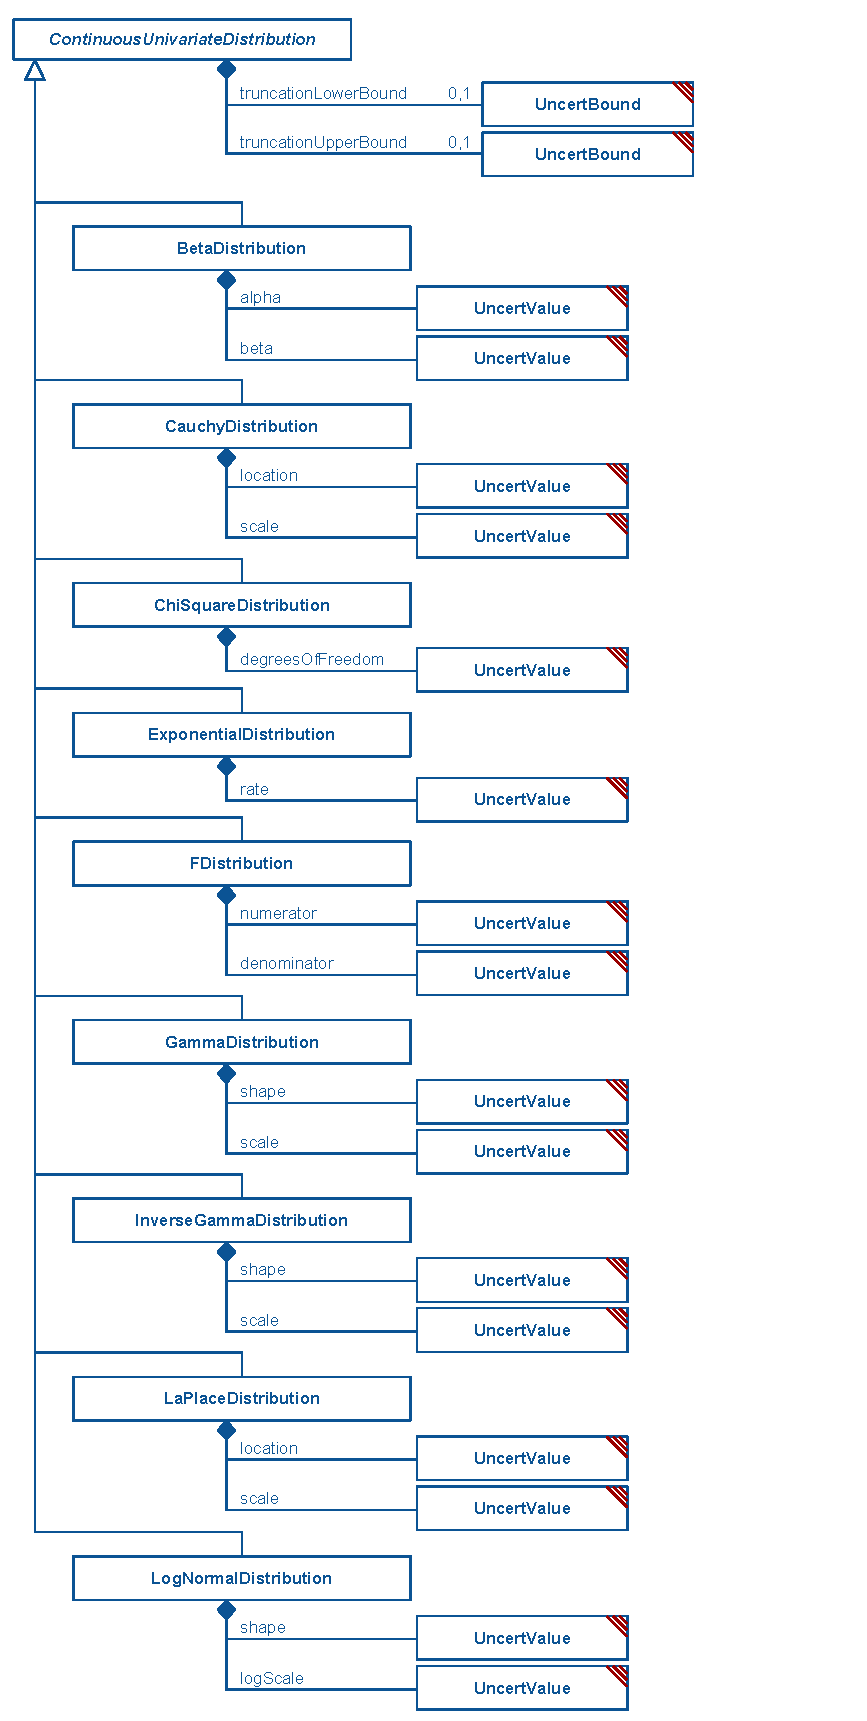
\includegraphics[width=0.55\linewidth]{figs/continuousUnivariateDistribution_first.pdf}
\caption{The definition of the \ContinuousUnivariateDistribution abstract class, and its \BetaDistribution, \CauchyDistribution, \ChiSquareDistribution, \ExponentialDistribution, \FDistribution, \GammaDistribution, \InverseGammaDistribution, \LaPlaceDistribution, and \LogNormalDistribution children.  All may have lower and upper \UncertBound children, and each has one or more other parameters encoded as \UncertValue children (both defined below).}
\label{fig:continuousUnivariateDistribution_first}
\end{figure}


\subsection{The \class{ContinuousUnivariateDistribution} class}
\label{ContinuousUnivariateDistribution-class}
\label{continuousunivariatedistribution-class}
The abstract \ContinuousUnivariateDistribution class is the base class for a wide variety of distributions, all of which describe a potentially-bounded continuous range of probabilities.  Many of the most commonly-used distributions such as the \NormalDistribution and the \UniformDistribution fall into this category.

\begin{figure}[htb]
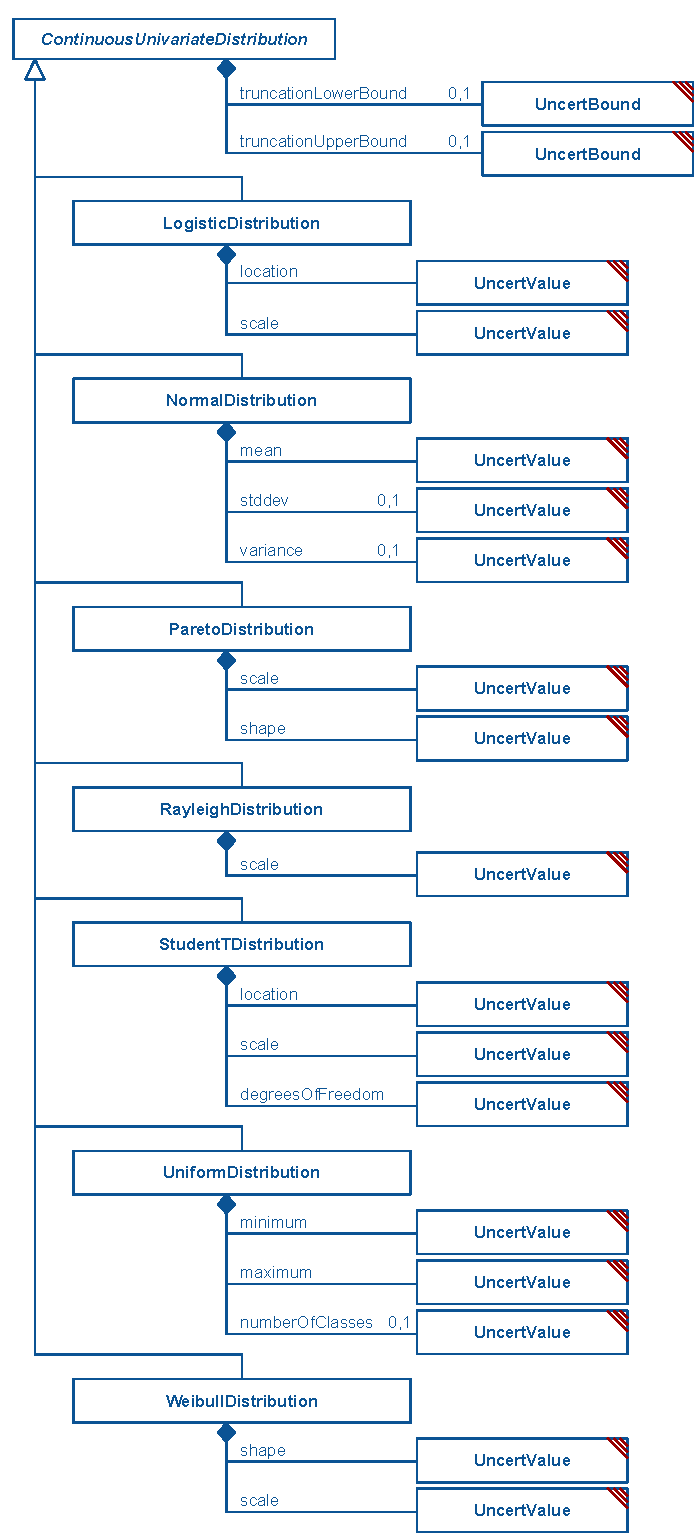
\includegraphics[width=0.55\linewidth]{figs/continuousUnivariateDistribution_second.pdf}
\caption{The definition of the \ContinuousUnivariateDistribution abstract class, and its \LogisticDistribution, \NormalDistribution, \ParetoDistribution, \RayleighDistribution, \StudentTDistribution, \UniformDistribution, and \WeibullDistribution children.  All may have lower and upper \UncertBound children, and each has one or more other parameters encoded as \UncertValue children (both defined below).}
\label{fig:continuousUnivariateDistribution_second}
\end{figure}

All \ContinuousUnivariateDistribution elements may have two optional children: \val{lowerTruncationBound} and \val{upperTruncationBound}, both of the class \UncertBound (defined below).  Either element, if present, limit the range of possible sampled values from the distribution.  The \val{lowerTruncationBound} defines the lowest value (inclusive or not, as defined by that element's \token{inclusive} attribute) that can be sampled, and the \val{upperTruncationBound} defines the highest.  If both children are present, the \val{lowerTruncationBound} must either be lower than the \val{upperTruncationBound}, or they may be equal, if both bounds are set \token{inclusive}=\val{true}.  Similarly, some distributions are themselves naturally bound (some may, for example, only return values greater than zero).  In those cases, the natural lower bound of the distribution must be either be lower than the \val{upperTruncationBound}, or be equal to it if the natural lower bound is inclusive, and if the \val{upperTruncationBound} is set \token{inclusive}=\val{true}.  Similarly, the natural upper bound of the distribution must either be higher than the \val{lowerTruncationBound}, or it may be equal to it if the natural upper bound is inclusive and if the \val{lowerTruncationBound} is set \token{inclusive}=\val{true}.  It may be impossible to determine this from a static analysis of the model, as either or both bound's values may depend on other dynamic variables.  If a simulator encounters this situation, the sampled value and the behavior of the simulator are undefined.

If bounded, the cumulative probability that would have been assigned to the region outside the bound is re-assigned proportionally to the rest of the distribution.  It should be noted that while discarding any value obtained from the non-truncated version of the distribution and re-sampling is indeed one method that could be used to accomplish this, the efficiency of that algorithm decreases with the width of the allowed window, and indeed is technically zero (and would take an infinite amount of time to complete) should the bounds be equal to one another.  Taking any samples obtained outside the bound window and instead returning the boundary value itself is incorrect, and will not result in a proper draw from the defined distribution.

The distributions of this type allowed in this version of the specification are defined in \fig{fig:continuousUnivariateDistribution_first} and \fig{fig:continuousUnivariateDistribution_second}.  A full list of all of the distributions is provided in \sec{sec:allDistributions}.


\begin{figure}[htb]
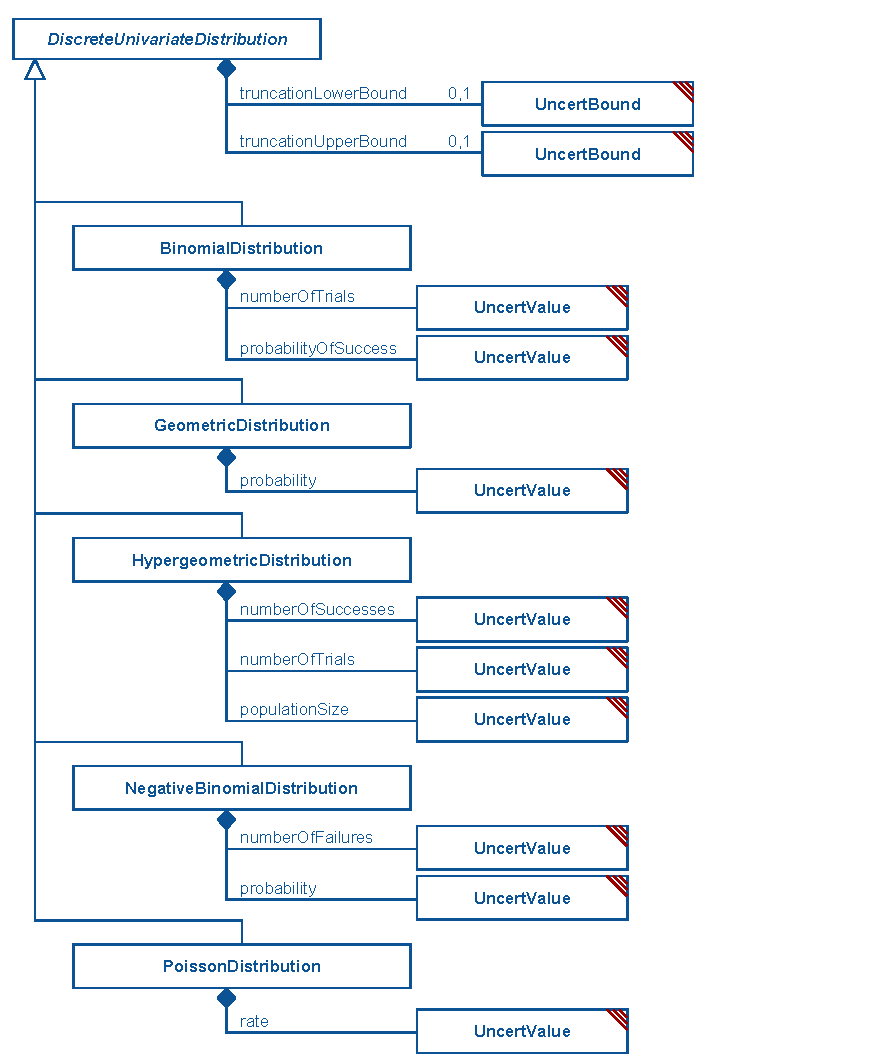
\includegraphics[width=0.55\linewidth]{figs/discreteUnivariateDistribution.pdf}
\caption{The definition of the \DiscreteUnivariateDistribution abstract class, and its \BinomialDistribution, \GeometricDistribution, \HypergeometricDistribution, \NegativeBinomialDistribution, and \PoissonDistribution children.  All may have lower and upper \UncertBound children, and each has one or more other parameters encoded as \UncertValue children (both defined below).}
\label{fig:discreteUnivariateDistribution}
\end{figure}

\subsection{The \class{DiscreteUnivariateDistribution} class}
\label{DiscreteUnivariateDistribution-class}
\label{discreteunivariatedistribution-class}

The abstract \DiscreteUnivariateDistribution class is the base class for a wide variety of distributions, all of which describe a potentially-bounded range of probabilities of discrete values.  The most commonly-used distributions in this class is probably the \PoissonDistribution.  Distributions that always return integers fall in this category, which often involve events happening at particular frequencies.

All \DiscreteUnivariateDistribution elements (like \ContinuousUnivariateDistribution elements) may have two optional children: \val{lowerTruncationBound} and \val{upperTruncationBound}, both of the class \UncertBound (defined below).  Either element, if present, limit the range of possible sampled values from the distribution.  The \val{lowerTruncationBound} defines the value below which no sampling may take place
(inclusive or not, as defined by that element's \token{inclusive} attribute), and the \val{upperTruncationBound} defines the value above which no sampling may take place.  These bounds may fall between the possible discrete values being returned:  as an example, for a distribution that returned an integer in the series [0, 1, 2, ...], if it was given a \val{lowerTruncationBound} of 1.5, the lowest value it could return would be 2.  In this case, the value of the \token{inclusive} attribute on the \UncertBound would be immaterial, as '1.5' could never be returned.

As in the case of the \ContinuousUnivariateDistribution bounds, if both bounds are present, the \val{lowerTruncationBound} must either be lower than the \val{upperTruncationBound}, or they may be equal, if both bounds are set \token{inclusive}=\val{true}.  Similarly, the discrete distributions are themselves often naturally bound (some may, for example, only return values greater than zero).  In those cases, the natural lower bound of the distribution must be either be lower than the \val{upperTruncationBound}, or it may be equal to it if the natural lower bound is inclusive, and if the \val{upperTruncationBound} is set \token{inclusive}=\val{true}.  Similarly, the natural upper bound of the distribution must either be higher than the \val{lowerTruncationBound}, or it may be equal to it if the natural upper bound is inclusive and if the \val{lowerTruncationBound} is set \token{inclusive}=\val{true}.  In addition, if both bounds are defined, they must define a span within which at least one possible sampled discrete value may be found.  For a distribution that returns integers, for example, one may not define a lower bound of 1.5 and an upper bound of 1.8, as no integer lies within that range.  It may be impossible to determine if any of these rules are violated from a static analysis of the model, as either or both bound's values may depend on other dynamic variables.  If a simulator encounters this situation, the sampled value and the behavior of the simulator are undefined.

If bounded, the cumulative probability that would have been assigned to the values outside the bound is re-assigned proportionally to the rest of the distribution.  It should be noted that while discarding any value obtained from the non-truncated version of the distribution and re-sampling is indeed one method that could be used to accomplish this, the efficiency of that algorithm decreases with the width of the allowed window, and indeed is technically zero (and could take an infinite amount of time to complete) should the bounds allow only a single discrete value.  Taking any samples obtained outside the bound window and instead returning the boundary value itself is incorrect, and will not result in a proper draw from the defined distribution.

The distributions of this type allowed in this version of the specification are defined in \fig{fig:discreteUnivariateDistribution}.  A full list of all of the distributions is provided in \sec{sec:allDistributions}.



\begin{figure}[htb]
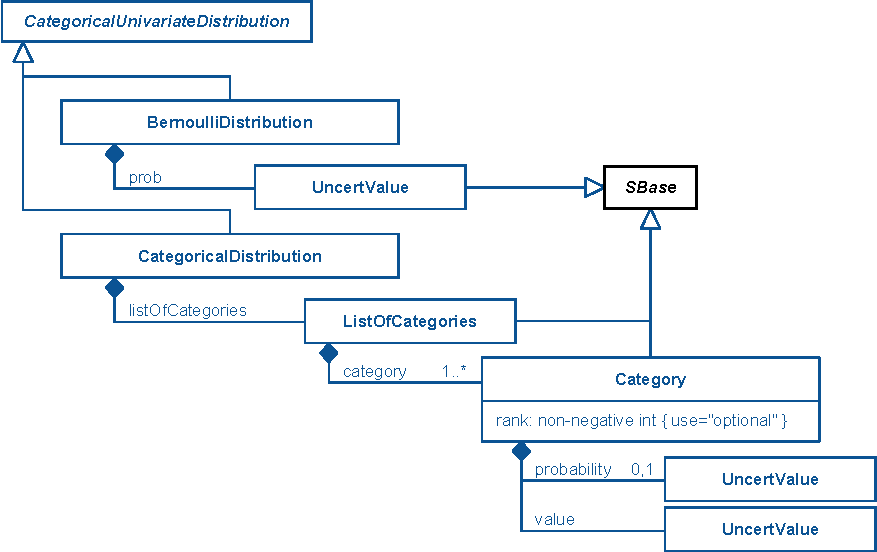
\includegraphics[width=0.85\linewidth]{figs/categoricalUnivariateDistribution.pdf}
\caption{The definition of the \CategoricalUnivariateDistribution abstract class, plus the \BernoulliDistribution, \CategoricalDistribution, \ListOfCategories, and \Category classes.}
\label{fig:categoricalUnivariateDistribution}
\end{figure}

\subsection{The \class{CategoricalUnivariateDistribution} class}
\label{CategoricalUnivariateDistribution-class}
\label{categoricalunivariatedistribution-class}

The \CategoricalUnivariateDistribution abstract class includes distributions where the various possible sampled values are each explicitly listed, along with the probability for that sampled value.  The sum of these probabilities must therefore equal 1.0, in order to be valid.  This type of distribution class is used for things such as weighted die rolls, or other situations where particular values are obtained at arbitrary probabilities.

Because each possible sampled value is explicitly listed in an \CategoricalUnivariateDistribution, it does not have the optional \UncertBound values that the other univariate distributions do: if a particular value is not allowed, it is simply dropped from the list of options, and the probabilities of the other values are scaled accordingly.


\subsection{Distribution Elements}

Because the list of distributions is extensive, all of them are provided at the end of this document in \sec{sec:allDistributions}.  The elements they use are defined below.

\begin{figure}[htb]
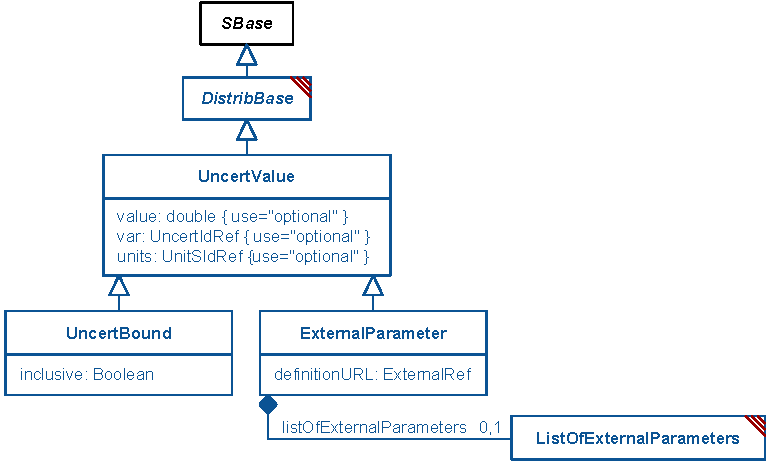
\includegraphics[width=0.35\linewidth]{figs/uncertValue.pdf}
\caption{The definition of the \UncertValue and \UncertBound classes.  These classes define a way to reference either a value or an element with mathematical meaning.  The \UncertBound class additionally defines whether it is considered to be inclusive or not.}
\label{fig:uncertValue}
\end{figure}

\subsubsection{The \class{UncertValue} class}
\label{UncertValue-class}
\label{uncertvalue-class}

The \UncertValue class provides two optional attributes, exactly one of which must be defined.  The \token{value} attribute (of type \primtype{double}) is used when the \UncertValue represents a particular number, and the \token{var} attribute (of type \primtype{UncertIdRef}) is used when the \UncertValue represents a referenced element with mathematical meaning.  In the context of a \FunctionDefinition, this can only reference a \DistribInput, as no \primtype{SId} from the \Model may be referenced from within a \FunctionDefinition.  In other contexts, it may reference the \primtype{SId} of any element with mathematical meaning; see \sec{sec:primtype-uncertidref}.

The optional \token{units} attribute may be used to indicate the units of the \token{val} attribute.  As such, it may only be defined if the \UncertValue has a defined \token{val} attribute, and not if it has a defined \token{var} attribute.  (In the latter case, the units may be derived from the referenced element.)

Any given \UncertValue in a \Distribution will have an element name specific to the parameter it represents within that \Distribution.  So, for example, a \NormalDistribution will have one child \UncertValue with the name \val{<mean>}, and might have another \UncertValue child with the name \val{<stddev>}.  All these parameters are defined as the same class for simplicity, since all of them merely need a way to reference a value.


\subsubsection{Attributes inherited from \SBase}

An \UncertValue always inherits the optional \token{metaid} and \token{sboTerm} attributes, and inherits optional \token{id} and \token{name} attributes as described in \sec{sec:idname}.  Outside of a \FunctionDefinition, the \token{id} of a \UncertValue takes the mathematical value of its \token{value} attribute if that attribute is defined, and the mathematical value of the corresponding \token{var} if that attribute is defined.  This meaning may be used in other contexts, but that meaning may not be set directly by any other SBML element of any level, version, or package.  If setting the value is desired, the \token{var} attribute should be used, and that referenced element set as per normal SBML procedures.  The meaning is provided mostly to allow access to the \token{val} attribute, which otherwise would be undiscoverable to any other SBML element.  Do note, however, that the scope of the \UncertValue \token{id} is limited to its \FunctionDefinition parent in that context.  In other contexts, its \token{id} has the scope of its parent \Model.

\subsubsection{The \class{UncertBound} class}
\label{UncertBound-class}
\label{uncertbound-class}

The \UncertBound class inherits from \UncertValue and adds a single required Boolean attribute \token{inclusive}.  This attribute indicates whether the value the bound represents is to be included in that range (\val{true}) or not (\val{false}).  This allows the creation of either 'open' or 'closed' boundaries of the ranges it is used to define.


\begin{figure}[htb]
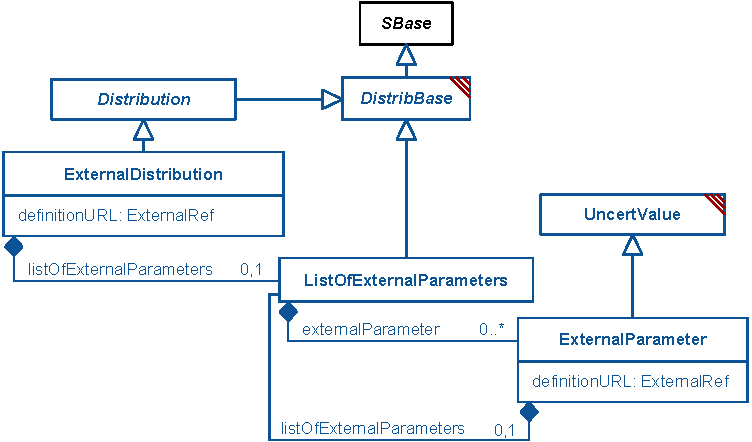
\includegraphics[width=0.85\linewidth]{figs/externalDistribution.pdf}
\caption{The definition of the \ExternalDistribution, \ExternalParameter, and \ListOfExternalParameters classes.  These classes define a way to define a distribution with reference to an external database or ontology of distribution definitions.}
\label{fig:externalDistribution}
\end{figure}

\subsection{The \class{ExternalDistribution} class}
\label{ExternalDistribution-class}
\label{externaldistribution-class}

The \ExternalDistribution class is provided to allow a modeler to encode a distribution not otherwise explicitly handled by this specification.  Because the range of possibilities is so vast, the modeler should not normally expect any given SBML simulator or other software to be able to properly manipulate this distribution, but particular software tools may implement support for certain distributions they know their own software's users may require.

The required attribute \token{definitionURL}, of type \primtype{ExternalRef}, must be a URI that defines a valid distribution.  It is strongly recommended that modelers use distributions from ProbOnto (\url{http://probonto.org/}), as consistently referencing a single ontology will improve exchangeability, at least slightly.  The referenced distribution is then the distribution defined by this \ExternalDistribution, along with any parameterization provided by the children \ExternalParameter elements.

Some referenced distributions are multivarite, meaning they define correlated distributions for two or more parameters.  It is impossible with \sbmlthreecore to define a \FunctionDefinition that returns a vector, and similarly no \primtype{SId} in \sbmlthreecore can be used to represent a vector.  If this is desired, then, the Arrays package must be used in concert with the \ExternalDistribution to cooperatively set up a model with a \FunctionDefinition that can use an array as input and/or as output.

The \ExternalDistribution defines an optional child \ListOfExternalParameters, which can be used to parameterize the defined distribution.


\subsection{The \class{ListOfExternalParameters} class}
\label{ListOfExternalParameters-class}
\label{listofexternalparameters-class}

The \ListOfExternalParameters class, like other \ListOf classes in \sbmlthreecore, is a container for zero or more \ExternalParameter objects.  If empty, it simply means that no child \ExternalParameter objects are defined for its parent, and is equivalent to not including the \ListOfExternalParameters object at all.  This situation might be useful if the list is annotated with the reason why it is empty, for example.


\subsection{The \class{ExternalParameter} class}
\label{ExternalParameter-class}
\label{externalparameter-class}

The \ExternalParameter class, like the \ExternalDistribution, is provided to allow a modeler to encode externally-provided parameters not otherwise explicitly handled by this specification.  Again, the range of possibilities is vast, so modelers should ensure that the tool they wish to use encodes support for any \ExternalParameter they define.

The \ExternalParameter inherits from \UncertValue, and adds the required attribute \token{definitionURL}, which is of type \primtype{ExternalRef}, and an optional child \ListOfExternalParameters.  The \token{definitionURL} must be a URI that defines a valid distribution-related parameter.  It is again strongly recommended that modelers use distribution parameters from ProbOnto (\url{http://probonto.org/}), as consistently referencing a single ontology will improve exchangeability.

The child \ListOfExternalParameters is provided because some parameters may themselves need further parameterization.  For example, a mixture distribution defined as an \ExternalDistribution would contain as child \ExternalParameter objects those other base distributions that were mixed in the overall distribution.  Those base distributions would need to define their own parameterization, which could be accomplished here with child \ExternalParameter objects.  Similarly, ranges or categories might also need to be further defined with reference to child \ExternalParameter objects that would be considered to 'belong' to the parent \ExternalParameter.

The referenced parameter is then the parameter defined by this \ExternalParameter, along with any further parameterization provided by its own children \ExternalParameter elements.

Some referenced distributions are multivarite, meaning they define correlated distributions for two or more parameters.  If an input \ExternalParameter is required for a distribution, one must use the inherited \token{var} attribute to define the parameter's value rather than the \token{value} attribute, and SBML must contain some way to define that referenced \token{var} as an array (such as the Arrays package).







%The full list of the 29 distributions and how they can be used is provided in \ref{sec:uncertml-distributions}.  Four of these distributions (Dirichlet, Multinomial, Multivariate Normal, and Multivariate Student T) use vectors as both input and output.  It is possible, if tedious, to provide vector input to these distributions by simply defining each element of the required vector as a numeric value or as an \primtype{UncertId.  However, it is not possible in \sbmlthreecore to take a single vector and simultaneously assign its values to different elements, or even to use a vector within MathML.  While it would be theoretically possible to define new elements in this specification to work around this limitation, such capabilities are more obviously the domain of the Arrays package within SBML, or of SED-ML\footnote{\url{http://sed-ml.org/}} (to set a suite of element values).  Unfortunately, as of this writing, the Arrays package has not yet been finalized, and many aspects of it have not been set.  Therefore, it is left to the future finalized Arrays package to define how to utilize a \FunctionDefinition that returns a vector, and how to define a \FunctionDefinition that takes a vector as input.  It is also possible for other individuals or groups to come up with custom annotations that define how to do this, and in fact, this is encouraged for any group that requires the use of any of these four distributions for their models.  If no such definitions exist, however, any numerical results from the use of these functions remain undefined, and models using this technique are unsimulatable.  (Such models may still be useful descriptions of certain situations, however.)  A final possibility is that SED-ML could be extended to extract the function definition, perform the sampling itself, and use the resulting vector to assign initial values to certain elements.

%All three Sample elements in UncertML are logistically identical, and only semantically different.  The RandomSample describes a set of realizations known to come from a randomly-distributed source.  The SystematicSample describes a set of deliberately chosen realizations, such as those resulting from unscented sampling methods for Gaussian random variables.  The UnknownSample describes a set of realizations for which the source distribution is unknown.  All three describe a set of realizations, each with a weight and one or more values. The weights of all realizations in a single Sample must sum to 1.0.

%UncertML also allows the definition of realizations with \val{categories} instead of \val{values} (i.e. \primtype{strings} instead of \primtype{doubles}).  This data type is unsupported in\sbmlthreecore, but if a package supports this data type in the future (as the Qualitative Models package might), \val{categories} could be used.

%When a \Distribution is encountered containing a Sample, its parent \FunctionDefinition is defined as randomly choosing a single realization from the the \uncertml according to its \token{weight}, and, if the realization contains a \token{values} child, returning that value (or vector of values) when the function is called.  If the realization contains a \token{categories} child, that string (or vector of strings) is returned instead.  (\uncertml requires that a single realization contain either a \token{values} or \token{categories} child, but may not have both.)

%As happens with some of the UncertML distributions above, then, if the chosen realization has multiple values or categories, the result of the draw is a vector, which cannot, in \sbmlthreecore, be used either in MathML or as an assignment to an SBML element.  The Arrays package or some form of custom annotation must be used to define what happens when a multi-value realization is chosen.

%Similarly, there is no \token{string} data type for SBML elements defined in \sbmlthreecore.  Without a package that defines such a data type, then, any call to a \FunctionDefinition that returns a string or vector of strings from a \token{categories} \uncertml element will be undefined and therefore unsimulatable, but may, again, be a useful description of a particular type of model.

%Note \notice that the \ExplicitPMF class in previous versions of this specification did not use \uncertml, and instead defined its own way of listing samples.  The functionality (with the addition of ids instead of numbers in \uncertml 3.0) is replicated in the CategoricalDistribution class of \uncertml 3.0.



\subsection{Discrete vs. continuous sampling}
\label{discrete-continuous}

The \primtype{SId}s of \FunctionDefinition elements can be used in \sbmlthreecore in both discrete and continuous contexts:  \InitialAssignment, \EventAssignment, \Priority, and \Delay elements are all discrete, while \Rule, \KineticLaw, and \Trigger elements are all continuous in time.  For discrete contexts, the behavior of \distribshort-extended \FunctionDefinition elements is well-defined:  one or more random values are sampled from the distribution each time the function definition is invoked. Each invocation implies one sampling operation.  In continuous contexts, however, their behavior is ill-defined.  More information than is defined in this package (such as autocorrelation values or full conditional probabilities) would be required to make random sampling tractable in continuous contexts, and is beyond the scope of this version of the package.  If some package is defined in the future that adds this information, or if custom annotations are provided that add this information, such models may become simulatable.  However, this package does not define how to handle sampling in continuous contexts, and recommends against it: a warning may be produced by any software encountering the use of a \distribshort-extended \FunctionDefinition in a continuous context.  Assuming such models are desirable, and the information is not provided in a separate package, this information may be incorporated into a future version of this specification.

Any other package that defines new contexts for MathML will also either be discrete or continuous.  Discrete situations (such as those defined in the Qualitative Models package) are, as above, well-defined.  Continuous situations (as might arise within the Spatial Processes package, over space instead of over time) will most likely be ill-defined.  Those packages must therefore either define for themselves how to handle \distribshort-extended \FunctionDefinition elements, or leave it to some other package/annotation scheme to define how to handle the situation.


%\subsection{Truncation}
%\label{truncation}

%In order to perform truncation, one or both ends of the distribution are cut off, and the remaining function is re-scaled so the area under the curve is once again 1.0.  This capability is provided through the use of the \val{truncationLowerBound} and \val{truncationUpperBound} elements.  As those element names imply, the first is used to truncate the distribution at a lower bound, and the second at an upper bound.  The fact that both are inclusive mean that the value at that boundary may possibly be returned by the function.  Care should thus be taken to ensure that (for example) if zero is a \emph{non-inclusive} bound for one's model, that a value slightly larger than zero be used as the distribution's inclusive lower bound.


\subsection{Examples using the extended \FunctionDefinition}
\label{sec:fd-examples}

Several examples are given below that illustrate various uses of an extended \FunctionDefinition.

\subsubsection{Defining and using a \NormalDistribution}
In the following example, a \FunctionDefinition is extended to define a draw from a \NormalDistribution:

\begin{example}
...
      <functionDefinition id="normal">
        <distrib:drawFromDistribution>
          <distrib:listOfDistribInputs>
            <distrib:distribInput distrib:id="mu" distrib:index="0"/>
            <distrib:distribInput distrib:id="sdev" distrib:index="1"/>
          </distrib:listOfDistribInputs>
          <distrib:normalDistribution>
            <distrib:mean distrib:var="mu"/>
            <distrib:stddev distrib:var="sdev"/>
          </distrib:normalDistribution>
        </distrib:drawFromDistribution>
      </functionDefinition>
...
\end{example}

Here, the \DistribInput children of \DrawFromDistribution define the local \primtype{UncertId}s \val{mu} and \val{sdev}, which are then used by the \Distribution as the \token{mean} and \token{stddev} of a normal distribution, as defined by UncertML.  (The example shown is from an SBML Level~3 Version~2 document, where the \token{<math>} child of a \FunctionDefinition is optional.) This function could then be used anywhere the \FunctionDefinition id \val{normal} can be used, as for example in an \InitialAssignment:

\begin{example}
...
    <initialAssignment symbol="y">
      <math xmlns="http://www.w3.org/1998/Math/MathML">
        <apply>
          <ci> normal </ci>
          <ci> z </ci>
          <cn> 10 </cn>
        </apply>
      </math>
    </initialAssignment>
...
\end{example}

This use would apply a draw from a normal distribution with mean \val{z} and standard deviation \val{10} to the SBML element \val{y}.

\subsubsection{Defining a truncated \NormalDistribution}
In the following example, a \FunctionDefinition is extended to define a draw from a truncated \NormalDistribution:

%Note: taken from stochastic test suite test 00073:
\begin{example}
...
      <functionDefinition id="normal_trunc">
        <distrib:drawFromDistribution>
          <distrib:listOfDistribInputs>
            <distrib:distribInput distrib:id="mean" distrib:index="0"/>
            <distrib:distribInput distrib:id="stddev" distrib:index="1"/>
            <distrib:distribInput distrib:id="lowerBound" distrib:index="2"/>
            <distrib:distribInput distrib:id="upperBound" distrib:index="3"/>
          </distrib:listOfDistribInputs>
          <distrib:normalDistribution>
            <distrib:truncationLowerBound distrib:var="lowerBound" distrib:inclusive="true"/>
            <distrib:truncationUpperBound distrib:var="upperBound" distrib:inclusive="true"/>
            <distrib:mean distrib:var="mean"/>
            <distrib:stddev distrib:var="stddev"/>
          </distrib:normalDistribution>
        </distrib:drawFromDistribution>
      </functionDefinition>
...
\end{example}

Here, the \DistribInput children of \DrawFromDistribution define four arguments: \token{mean}, \token{stddev}, \token{lowerBound}, and \token{upperBound}.  These arguments are then used as the values of the \token{var} attributes of the corresponding \UncertValue children of the \NormalDistribution.  An example use in an \InitialAssignment might look like:

\begin{example}
...
      <initialAssignment symbol="y">
        <math xmlns="http://www.w3.org/1998/Math/MathML">
          <apply>
            <ci> normal_trunc </ci>
            <ci> z </ci>
            <cn type="integer"> 10 </cn>
            <apply>
              <minus/>
              <ci> z </ci>
              <cn type="integer"> 2 </cn>
            </apply>
            <apply>
              <plus/>
              <ci> z </ci>
              <cn type="integer"> 2 </cn>
            </apply>
          </apply>
        </math>
      </initialAssignment>
...
\end{example}

This use would apply a draw from a normal distribution with mean $z$, standard deviation $10$, lower bound $z-2$ and upper bound $z+2$ (inclusive) to the SBML element \val{y}.


\subsubsection{Defining a 'die roll' PMF with a \CategoricalDistribution}
In the following example, a \FunctionDefinition is extended to define a draw from a \CategoricalDistribution PMF:

%\clearpage
\begin{example}
...
      <functionDefinition id="die_roll">
        <distrib:drawFromDistribution>
          <distrib:categoricalDistribution>
            <distrib:listOfCategories>
              <distrib:category>
                <distrib:probability distrib:value="0.25"/>
                <distrib:value distrib:value="1"/>
              </distrib:category>
              <distrib:category>
                <distrib:probability distrib:value="0.25"/>
                <distrib:value distrib:value="2"/>
              </distrib:category>
              <distrib:category>
                <distrib:probability distrib:value="0.25"/>
                <distrib:value distrib:value="3"/>
              </distrib:category>
              <distrib:category>
                <distrib:value distrib:value="4"/>
              </distrib:category>
            </distrib:listOfCategories>
          </distrib:categoricalDistribution>
        </distrib:drawFromDistribution>
      </functionDefinition>
...
\end{example}

No inputs are provided.  Three of the four \Category children of the \CategoricalDistribution all have equal values for their \token{probability} children, with the fourth not having its probability set, meaning that it has a probability such that the sum of all the probabilities among all categories is 1.0.  Each child \Category is therefore equally likely to be chosen, resulting in this function returning \val{1}, \val{2}, \val{3}, or \val{4}, each with equal probability.

In a modeling context where it is not a die being rolled, but different patients which we are sampling, the following function definition uses the same structure:

\begin{example}
...
      <functionDefinition id="pick_patient">
        <distrib:drawFromDistribution>
          <distrib:categoricalDistribution>
            <distrib:listOfCategories>
              <distrib:category id="patient1">
                <distrib:probability distrib:value="0.25"/>
                <distrib:value distrib:value="1.21"/>
              </distrib:category>
              <distrib:category id="patient2">
                <distrib:probability distrib:value="0.25"/>
                <distrib:value distrib:value="2.24"/>
              </distrib:category>
              <distrib:category id="patient3">
                <distrib:probability distrib:value="0.25"/>
                <distrib:value distrib:value="-0.6"/>
              </distrib:category>
              <distrib:category id="patient4">
                <distrib:value distrib:value="1.82"/>
              </distrib:category>
            </distrib:listOfCategories>
          </distrib:categoricalDistribution>
        </distrib:drawFromDistribution>
      </functionDefinition>
...
\end{example}

Here, we have four patients, each of which had a different value.  When sampled (such as in an initial assignment), one would be chosen at random to populate a value for the simulation.  In a more complicated context where several different values were sampled from a single patient, the 'Arrays' package would need to be used, so that all the values from a single patient could be returned as a group, and then assigned to their appropriate targets.  In that case, various arrays could be set up with the first value in all arrays corresponding to the first patient, the second value with the second patient, etc.  A \DrawFromDistribution could then be created to return a patient index at random, and that index used to assign values in the simulation.


\subsubsection{Defining an external distribution}

In the following example, a \FunctionDefinition is extended to define a draw from an externally-defined distribution (in this case, an alternative parameterization of the \ExponentialDistribution):

\begin{example}
...
      <functionDefinition id="Exponential2">
        <distrib:drawFromDistribution>
          <distrib:listOfDistribInputs>
            <distrib:distribInput id="beta" distrib:index="0"/>
          </distrib:listOfDistribInputs>
          <distrib:externalDistribution name="Exponential 2"
              distrib:definitionURL="http://www.probonto.org/ontology#PROB_k0000353">
            <distrib:listOfExternalParameters>
              <distrib:externalParameter name="Beta" distrib:var="beta"
                distrib:definitionURL="http://www.probonto.org/ontology#PROB_k0000362"/>
            </distrib:listOfExternalParameters>
          </distrib:externalDistribution>
        </distrib:drawFromDistribution>
      </functionDefinition>
...
\end{example}

As defined in the ProbOnto ontology, this parameterization of the exponential distribution takes the form $1/{\beta e^{-x/\beta}}$ instead of the form $\lambda e^{-x\lambda}$, used by the \ExponentialDistribution.  







%\subsubsection{Defining a 'pick one' sample with UncertML}
%In the following example, a \FunctionDefinition is extended to define a draw from an UncertML-defined set of samples:

%\begin{example}
%<sbml xmlns:distrib="http://www.sbml.org/sbml/level3/distrib/version1" xmlns="http://www.sbml.org/sbml/level3/version2/core" level="3" version="2" distrib:required="true">
%  <model>
%    <listOfFunctionDefinitions>
%      <functionDefinition id="pick_one">
%        <distrib:drawFromDistribution>
%          <distrib:listOfDistribInputs>
%            <distrib:distribInput distrib:id="A" distrib:index="0"/>
%            <distrib:distribInput distrib:id="B" distrib:index="1"/>
%            <distrib:distribInput distrib:id="C" distrib:index="2"/>
%            <distrib:distribInput distrib:id="D" distrib:index="3"/>
%          </distrib:listOfDistribInputs>
%          <distrib:categoricalDistribution>
%            <distrib:listOfCategories>
%              <distrib:category>
%                <distrib:probability distrib:value="0.25"/>
%                <distrib:value distrib:var="A"/>
%              </distrib:category>
%              <distrib:category>
%                <distrib:probability distrib:value="0.25"/>
%                <distrib:value distrib:var="B"/>
%              </distrib:category>
%              <distrib:category>
%                <distrib:probability distrib:value="0.25"/>
%                <distrib:value distrib:var="C"/>
%              </distrib:category>
%              <distrib:category>
%                <distrib:value distrib:var="D"/>
%              </distrib:category>
%            </distrib:listOfCategories>
%          </distrib:categoricalDistribution>
%        </distrib:drawFromDistribution>
%      </functionDefinition>
%    </listOfFunctionDefinitions>
%    <listOfParameters>
%      <parameter id="y"/>
%    </listOfParameters>
%    <listOfInitialAssignments>
%      <initialAssignment symbol="y">
%        <math xmlns="http://www.w3.org/1998/Math/MathML">
%          <apply>
%          <apply>
%            <ci> pick_one </ci>
%            <cn> 0.3 </cn>
%            <cn> 5.2 </cn>
%            <cn> -4 </cn>
%            <cn> 8.77 </cn>
%          </apply>
%        </math>
%      </initialAssignment>
%    </listOfInitialAssignments>
%  </model>
%</sbml>
%\end{example}

%In this example, the function 'pickone' is defined, with four arguments, \val{A}, \val{B}, \val{C}, and \val{D}.  When called, each argument has an equal chance of being chosen as the return value.  The parameter 'x' is initialized by calling this function with the arguments 0.3, 5.2, -4, and 8.77, each of which has an equally likely chance of being chosen.


\subsection{Equivalence with Fallback Function}
\label{sec:fallbackfunc}

The \mathml definition directly contained by the
\class{functionDefinition} is not used, but is required by \threeone.  (It is optional in \threetwo.)  To ensure the continued validity of the model, the following rules must be followed:

\begin{itemize}
\item The lambda function should have the same number of arguments as
  its equivalent distribution (defined by \distribshort).
\item Each argument should match the type of the equivalent argument
  in the external function.
\item The lambda function should have the same return type as the
  \emph{sampled} distribution. For example, if a predefined PDF when
  sampled returns a scalar value, the dummy function should also do so.
\end{itemize}

Clearly, these rules can only be enforced by a \distribshort-aware validator.

In the following example, the fallback function is coded to simply return \val{mean}, the first argument of the function.  Note that the arguments have been given different local ids (\val{mean} and \val{s} instead of \val{avg} and \val{sdev}); their equivalence is based on order, not string matching.

\begin{example}
      <functionDefinition id="normal">
        <math xmlns="http://www.w3.org/1998/Math/MathML">
          <lambda>
            <bvar>
              <ci> mean </ci>
            </bvar>
            <bvar>
              <ci> sdev </ci>
            </bvar>
            <ci> mean </ci>
          </lambda>
        </math>
        <distrib:drawFromDistribution>
          <distrib:listOfDistribInputs>
            <distrib:distribInput distrib:id="mean" distrib:index="0"/>
            <distrib:distribInput distrib:id="s" distrib:index="1"/>
          </distrib:listOfDistribInputs>
          <distrib:normalDistribution>
            <distrib:mean distrib:var="mean"/>
            <distrib:stddev distrib:var="s"/>
          </distrib:normalDistribution>
        </distrib:drawFromDistribution>
      </functionDefinition>
\end{example}

\begin{figure}[bh]
  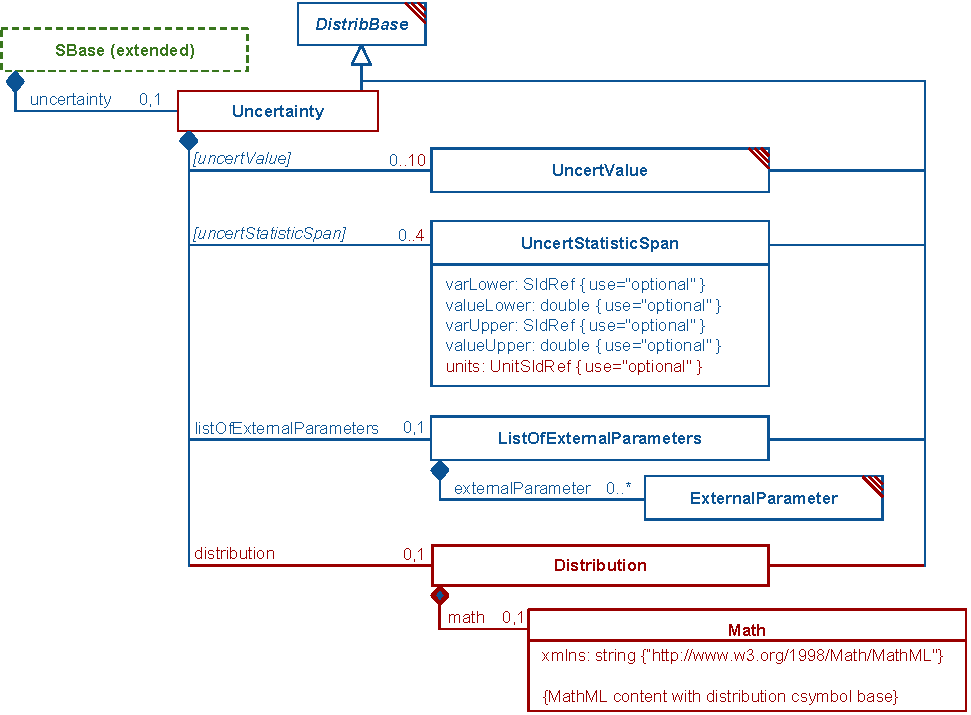
\includegraphics{figs/extended-sbase.pdf}
  \caption{The definition of the extended \SBase class to include a new optional \Uncertainty child, which in turn has optional \UncertStatistics and \Distribution children.  Intended for use with any element with mathematical meaning, or with a \Math child.}
  \label{fig:extended-sbase-uml}
\end{figure}

\subsection{The extended \SBase class}
\label{sec:extended-sbase-class}
\label{extended-sbase-class}

As can be seen in \fig{fig:extended-sbase-uml}, the SBML base class \SBase is extended to include an optional \Uncertainty child, which in turn contains an optional \Distribution child, and an optional \UncertStatistics child, either or both of which may be used to include information about the uncertainty of the parent element.  In \sbmlthreecore, one should only extend those \SBase elements with mathematical meaning (so, \Compartment, \Parameter, \Reaction, \Species, and \SpeciesReference), or those \SBase elements with \Math children (so, \Constraint, \Delay, \EventAssignment, \FunctionDefinition, \InitialAssignment, \KineticLaw, \Priority, \Rule, and \Trigger).  These are added here to \SBase instead of to each of these the various SBML elements so that other packages inherit the ability to extend their own elements in the same fashion:  for example, the \FluxBound class from the Flux Balance Constraints package has mathematical meaning, and could be given information about the distribution or set of samples from which it was drawn.  Similarly, the \FunctionTerm class from the Qualitative Models package has a \Math child, and could be similarly extended.

A few SBML elements can interact in interesting ways that can confuse the semantics here.  A \Reaction element and its \KineticLaw child, for example, both reference the exact same mathematics, so only one should be extended with a child \Distribution and/or \UncertStatistics.  Similarly, if an \InitialAssignment assigns to a constant element (\Parameter, \Species, etc.), the uncertainty for both should be the same, or only one should be provided.

Other elements not listed above should probably not be given an \Uncertainty child, as it would normally not make sense to talk about the uncertainty of something that doesn't have a corresponding mathematical meaning.  However, because packages or annotations can theoretically give new meaning (including mathematical meaning) to elements that previously did not have them, this is not a requirement.

It is important to note that the uncertainty described either by the \Distribution or the \UncertStatistics elements are defined as being the uncertainty at the moment the element's mathematical meaning is calculated, and does not describe the uncertainty of how that element changes over time.  For a \Species, \Parameter, \Compartment, and \SpeciesReference, this means that it is the uncertainty of their initial values, and does not describe the uncertainty in how those values evolve in time.  The reason for this is that other SBML constructs all describe how (or if) the values change in time, and it is those other constructs that should be used to describe a symbol's time-based uncertainty.  For example, a \Species whose initial value had uncertainty due to instrument precision could have an \Uncertainty child describing this.  A \Species whose value was known to change over time due to unknown processes, but which had a known average and standard deviation could be given an \AssignmentRule that set that \Species amount to the known average, and the \AssignmentRule itself could be given an \UncertStatistics child describing the standard deviation of the variability.


\subsection{The \class{Uncertainty} class}
\label{Uncertainty-class}
\label{uncertainty-class}

The \Uncertainty class has two optional children: an \UncertStatistics child and a \Distribution child.  Either or both may be used, depending on the information about the parent that the modeler wishes to store in this object.  If neither is present, this means that no information about the uncertainty of the object is provided by this package.  The \Uncertainty may be annotated to provide more information about why this is.

Note that the described uncertainty for elements that change in value over time apply only to the element's uncertainty at a snapshot in time, and not the uncertainty in how it changes in time.  For typical simulations, this means the element's initial condition.  Note too that the description of the uncertainty of a \Species should describe the uncertainty of its \token{amount}, not the uncertainty of its \token{concentration}.  The 'primary' mathematical meaning of a \Species in SBML is always the amount; the concentration may be used, but is considered to be derived.

\subsubsection{Attributes inherited from \SBase}

An \Uncertainty always inherits the optional \token{metaid} and \token{sboTerm} attributes, and inherits optional \token{id} and \token{name} attributes as described in \sec{sec:idname}.  The \token{id} of an \Uncertainty has no mathematical meaning.

\begin{figure}[bh]
  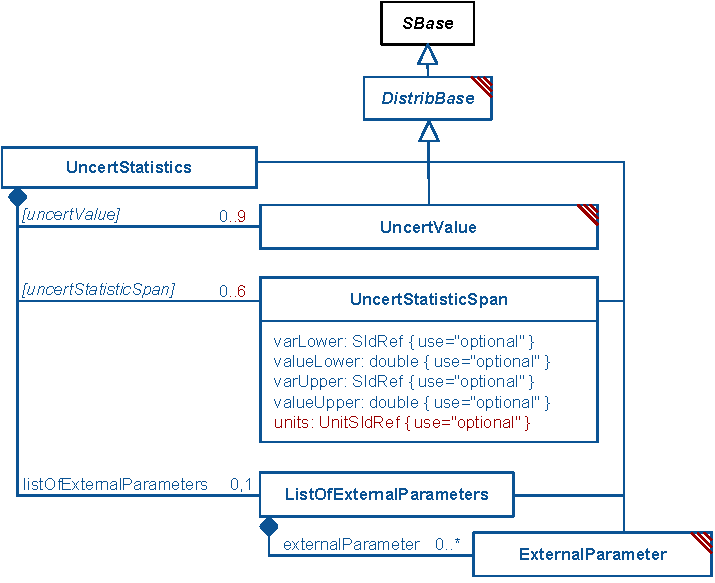
\includegraphics{figs/uncertStatistics.pdf}
  \caption{The definition of the \UncertStatistics and \UncertStatisticSpan classes.  (The \UncertValue and \ExternalParameter classes are defined elsewhere and re-used here.)  The \UncertStatistics class actually has a number of optional children, in three groups: those that can be classified as 'single value' statistics, those that can be classified as a 'span', and those not defined in this specification, but by an external ontology such as ProbOnto.  The possible 'single value' statistics are listed in \sec{UncertStatistics-class}}
  \label{fig:uncertStatistics}
\end{figure}


\subsection{The \class{UncertStatistics} class}
\label{UncertStatistics-class}
\label{uncertstatistics-class}

The \UncertStatistics class is a collection of zero or more statistical measures related to the uncertainty of the parent SBML element.  It contains three types of children:  \UncertValue children and \UncertStatisticSpan children, distinguished from each other by the element name of that child (listed below), and a \ListOfExternalParameters child, which contains zero or more \ExternalParameter objects.

The possible \UncertValue children are listed below.  Each is defined by its element name; the mean would be defined as \token{<mean>}, the standard deviation as \token{<standardDeviation>}, etc.

All the definitions below are from an archived copy of the definitions at \url{http://uncertml.org/}.

\begin{itemize}

\item \token{coefficientOfVariation}:  For a random variable with mean $ \mu $ and strictly positive standard deviation $ \sigma $, the coefficient of variation is defined as the ratio $ \frac{\sigma}{\mid\mu\mid} $. One benefit of using the coefficient of variation rather than the standard deviation is that it is unitless.

\item \token{kurtosis}:  The kurtosis of a distribution is a measure of how peaked the distribution is. The kurtosis is defined as $  \frac{\mu_4}{\sigma^4} $ where $ \mu_4 $ is the fourth centred moment of the distribution and $ \sigma $ is its standard deviation.

\item \token{mean}:  The arithmetic mean (typically just the mean) is what is commonly called the average. It is defined as $ \bar{x} = \frac{1}{n}\cdot \sum_{i=1}^n{x_i} $ where $ x_i $ represents with $ i $th observation of the quantity $ x $ in the sample set of size $ n $. It is related to the expected value of a random variable, $ \mu = E[X] $ in that the population mean, $ \mu $, which is the average of all quantities in the population and is typically not known, is replaced by its estimator, the sample mean $ \bar{x} $. Note that this statistic does not deal with issues of sample size, rather the mean is taken to refer to the population mean.

\item \token{median}:  The median is described as the numeric value separating the higher half of a sample (or population) from the lower half. The median of a finite list of numbers can be found by arranging all the observations from lowest value to highest value and picking the middle one. If there is an even number of observations, then there is no single middle value, then the average of the two middle values is used. The median is also the 0.5 quantile, or 50th percentile.

\item \token{mode}:  The mode is the value that occurs the most frequently in a data set (or a probability distribution). It need not be unique (e.g. two or more quantities occur equally often) and is typically defined for continuous valued quantities by first defining the histogram, and then giving the central value of the bin containing the most counts.

\item \token{skewness}:  The skewness of a random variable is a measure of how asymmetric the corresponding probability distribution is. The skewness is defined as $  \frac{\mu_3}{\sigma^3} $ where $ \mu_3 $ is the 3rd centred moment of the distribution and $ \sigma $ is its standard deviation.

\item \token{standardDeviation}:  The standard deviation of a  distribution or population is the square root of its variance and is given by $ \sigma = \sqrt{E[(X - \mu)^2]} $ where $ \mu = E[X] $. The population standard deviation is given by $ \sigma = \sqrt{\frac{1}{n} \sum_{i=1}^n\left(x_i - \bar{x} \right)^2} $ where $ \bar{x} = \frac{1}{n}\cdot \sum_{i=1}^n{x_i} $, $ x_i $ represents with $ i $th observation of the quantity $ x $ in the population of size $ n $. The standard deviation is a widely used measure of the variability or dispersion since it is reported in the natural units of the quantity being considered. Note that if a finite sample of a population has been used then the sample standard deviation is the appropriate unbiased estimator to use.

\item \token{variance}:  The variance of a random quantity (or distribution) is the average value of the square of the deviation of that variable from its mean, given by $ \sigma^2 = Var[X] = E[(X - \mu)^2] $ where $ \mu = E[X] $. The complete population variance is given by $ \sigma^2 = \frac{1}{n} \sum_{i=1}^n\left(x_i - \bar{x} \right)^2 $ where $ \bar{x} = \frac{1}{n}\cdot \sum_{i=1}^n{x_i} $, $ x_i $ represents with $ i $th observation of the quantity $ x $ in the population of size $ n $. This is the estimator of the population variance and should be replaced by the sample variance when using samples of finite size.


\end{itemize}

The possible \UncertStatisticSpan children are similar, defining a bounded span of values instead of a single value:

\begin{itemize}

\item {\token{confidenceInterval}:  For a univariate random variable $ x $, a confidence interval is a range $ [a,b] $, $ a<b $, so that $ x $ lies between $ a $ and $ b $ with given probability. For example, a 95\% confidence interval is a range in which $ x $ falls 95\% of the time (or with probability 0.95). Confidence intervals provide intuitive summaries of the statistics of the variable $ x $.

If $ x $ has a continuous probability distribution $ P $, then $ [a,b] $ is a 95\% confidence interval if $ \int_a^b P(x) = 0.95 $.

Unless specified otherwise, the confidence interval is usually chosen so that the remaining probability is split equally, that is $ P(x<a) = P(x>b) $. If $ x $ has a symmetric distribution, then the confidence intervals are usually centred around the mean. However, non-centred confidence intervals are possible and are better described by their lower and upper quantiles or levels. For example, a 50\% confidence interval would usually lie between the 25\% and 75\% quantiles, but could in theory also lie between the 10\% and 60\% quantiles, although this would be rare in practice. The \token{confidenceInterval} allows you the flexibility to specify non-symmetric confidence intervals however in practice we would expect the main usage to be for symmetric intervals.

The \token{confidenceInterval} child of a \UncertStatistics is always the 95\% confidence interval.  For other confidence intervals, use an \ExternalParameter instead. }

\item {\token{credibleInterval}:  In Bayesian statistics, a credible interval is similar to a confidence interval determined from the posterior distribution of a random variable $ x $. That is, given a prior distribution $ p(x) $ and some observations $ D $, the posterior probability $ p(x\mid D) $ can be computed using Bayes theorem. A 95\% credible interval is then any interval $ [a,b] $ so that $ \int_a^b p(x\mid D) = 0.95 $, that is the variable $ x $ lies in the interval $ [a,b] $ with posterior probability 0.95. Note that the interpretation of a credible interval is not the same as a (frequentist) confidence interval.

The \token{credibleInterval} child of a \UncertStatistics is always the 95\% credible interval.  For other credibility intervals, use an \ExternalParameter instead.}


\item \token{interquartileRange}:  The interquartile range is the range between the 1st and 3rd quartiles. It contains the middle 50\% of the sample realisations (or of the sample probability). It is typically used and shown in box plots.

\item \token{range}:  The range is the interval $ [a,b] $ so that $ a<b $ and contains all possible values of $ x $. This is also often called the statistical range, which is the distance from the smallest value to the largest value in a sample dataset. For a sample dataset $ X = (x_1, ..., x_N $), the range is the distance from the smallest $ x_i $ to the largest. It is often used as a first estimate of the sample dispersion.

\end{itemize}

Any number of \ExternalParameter children may be included as well, each defined by its \token{definitionURL}.  

The following statistics could be added to \UncertStatistics fairly straightforwardly, but are not in the current version, since each is defined not by a single value, but by at least two, and are not defined by a range.  If any of the following are desired, they can be added to a subsequent version.  Note that is is possible to encode them in the current version though the use of the \ExternalParameter construct, though no ontology is known currently that defines these elements (ProbOnto is solely for distributions, and does not encompass statistical measures.  UncertML did include them, and though it is now defunct, the old URLs could still be used if desired.)

\begin{itemize}
\item \token{centredMoment}:  For a given positive natural number $ k $, the $ k\textsuperscript{th} $ central moment of a random variable $ x $ is defined as $ \mu_k = E[(x - E[x])^k] $. That is, it is the expected value of the deviation from the mean to the power $ k $. In particular, $ \mu_0 = 1 $, $ \mu_1 = 0 $ and $ \mu_2 $ is the variance of $ x $.

\item \token{correlation}:  The correlation between two random variables $ x_1 $ and $ x_2 $ is the extent to which these variable vary together in a linear fashion. It is characterised by the coefficient $ \rho_{1,2} = \frac{E[(x_1-\mu_1)(x_2-\mu_2)]}{\sigma_1\sigma_2} $ where $ \mu_1 $ and $ \mu_2 $ are the means of $ x_1 $ and $ x_2 $ respectively, and $ \sigma_1 $ and $ \sigma_2 $ are their respective standard deviations. Note this is strictly not a description of uncertainty, but it can be useful to represent the correlation between two variables. Generally a covariance specification would be preferred since this describes the uncertainty.

\item \token{decile}:  A decile, $ d $, is any of the nine values that divide the sorted quantities into ten equal parts, so that each part represents 1/10 of the sample, population or distribution. The first decile is equivalent to the 10th percentile.

\item \token{moment}:  For a given positive natural number $ k $, the $ k\textsuperscript{th} $ moment of a random variable $ x $ is defined as $ \mu_k = E[x^k] $. In particular, $ \mu_0 = 1 $ and $ \mu_1 $ is the mean of $ x $.
The moments can be defined with respect to some point $ a $, that is $ \mu_k(a) = E[(x - a)^k] $. Moments defined about the mean are called centred moments.

\item \token{percentile}:  A percentile is the value of a quantity below which a certain percent of values fall. This can be defined for samples, populations and distributions. For finite samples there is no widely accepted method, but all methods essentially rank the quantities and then use some interpolation to compute the percentile, unless the sample size $ n $ is a multiple of 100. For probability distributions the inverse cumulative density function can be used.  The most widely used method is as follows: to estimate the value, $ x_p $, of the $ p $th percentile of an ascending ordered dataset containing $ n $ elements with values $ x_1, x_2, ... ,x_n $ first compute $ \rho = \frac{p}{100}\,({n}-1)+1 $. Now $ \rho $ is split into its integer component, $ k $, and decimal component, $ d $, such that $ \rho = k + d $. $ x_p $ is then calculated as $ x_p = x_k+d(x_{k+1}-x_k) $ where $ 1 < \rho < n $ with special cases $ x_p = x_1 \; [\rho=1]; \ x_n \; [\rho=n] $.

\item \token{probability}:  Given a random variable $ x $ with probability density function $ f(x) $, the probability that $ x $ lies in some part of its domain $ \mathcal{X} $ is defined as $ P(x \in \mathcal{X}) = \int_{x\in\mathcal{X}} f(x) $. $ \mathcal{X} $ can be defined as a lower- or upper-bounded range, e.g. $ P(x < 3.2) $ or as the intersection of several such ranges, e.g. $ P(x \geq 1.7 \cap x < 3.2) $.

\item \token{quantile}:  Given a random variable $ x $, the $ n $-quantiles are the values of $ x $ which split the domain into $ n $ regions of equal probability. For instance, the $ k\textsuperscript{th} $ $ n $-quantile is the value $ q_k $ for which $ P(x<q_k) = \frac{k}{n} $. For some common values of $ n $, the $ n $-quantiles have additional names, namely quartiles for $ n=4 $, deciles for $ n=10 $ and percentiles for $ n=100 $.
More generally, a quantile can be associated to any probability $ p $, so that $ q $ is the value of $ x $ below which a proportion $ p $ of the probability lies, i.e. $ P(x<q) = p $.
The plot on the right shows the 1st to 9th 10-quantiles (or deciles) for a normal distribution ($ \mu = 4 $, $ \sigma = 1 $) as orange dots. The blue curve is the cumulative density function of $ x $. Note how the quantiles split the probability (y-axis) into 10 equal regions.

\item \token{quartile}:  The quartiles are the 4-quantiles, that is the 4 values of $ x $ below which lies a proportion 0.25, 0.50, 0.75 and 1 of the probability. One can also think of them as the 4 values of $ x $ which split the domain into 4 regions of equal probability.
\end{itemize}

\subsubsection{Attributes inherited from \SBase}

An \UncertStatistics always inherits the optional \token{metaid} and \token{sboTerm} attributes, and inherits optional \token{id} and \token{name} attributes as described in \sec{sec:idname}.  The \token{id} of an \UncertStatistics has no mathematical meaning.


\subsection{The \class{UncertStatisticSpan} class}
\label{UncertStatisticSpan-class}
\label{uncertstatisticspan-class}

The \UncertStatisticSpan class defines a span of values that define an uncertainty statistic such as confidence interval or range.  It has four optional attributes, \token{varLower} and \token{varUpper}, of type \primtype{SIdRef}, and \token{valueLower} and \token{valueUpper}, of type double.  Exactly one of the attributes \token{varLower} and \token{vaueLower} may be defined, and exactly one of the attributes \token{varUpper} and \token{valueUpper} may be defined.  If no attributes are defined, the parameters of the span are undefined.  If only one attribute is defined (one of the upper or lower attributes), that aspect of the span is defined, and the other end is undefined.  The span is fully defined if two attributes (one lower and one upper) is defined.

The value of the lower attribute (whichever is defined) must be lesser or equal to the value of the upper attribute (whichever is defined), at the initial conditions of the model.  The \UncertStatistics element cannot affect the core mathematics of an SBML model, but if it is used in a mathematical context during simulation of the model, this restriction on the attribute values must be maintained, or the \UncertStatisticSpan object as a whole will be undefined.

\subsubsection{Attributes inherited from \SBase}

An \UncertStatisticSpan always inherits the optional \token{metaid} and \token{sboTerm} attributes, and inherits optional \token{id} and \token{name} attributes as described in \sec{sec:idname}.  The \token{id} of an \UncertStatisticSpan has no mathematical meaning.


%The optional \token{id} attribute on the \Uncertainty object class serves to provide a way to identify the uncertainty.  The attribute takes a value of type \primtype{SId}.  Note that the identifier of a the uncertainty carries no mathematical interpretation and cannot be used in mathematical formulas in a model.  \Uncertainty also has an optional \token{name} attribute, of type \primtype{string}.  The \token{name} attribute may be used in the same manner as other \token{name} attributes on \sbmlthreecore objects; please see Section~3.3.2 of the \sbmlthreecore specification for more information.




\subsection{Examples using extended \SBase}
\label{extended-sbase-examples}

Several examples are given to illustrate the use of the \Uncertainty class:


\subsubsection{Basic \Uncertainty example}

In this examples, a species is given an \Uncertainty child to describe its standard deviation:

\begin{example}
...
      <species id="s1" compartment="C" initialAmount="3.22" hasOnlySubstanceUnits="true"
               boundaryCondition="false" constant="false">
        <distrib:uncertainty>
          <distrib:uncertStatistics>
            <distrib:standardDeviation distrib:value="0.3"/>
          </distrib:uncertStatistics>
        </distrib:uncertainty>
      </species>
...
\end{example}

Here, the species with an initial amount of 3.22 is described as having a standard deviation of 0.3, a value that might be written as \val{3.22 $\pm$ 0.3}.  This is probably the simplest way to use the package to introduce facts about the uncertainty of the measurements of the values present in the model.

It is also possible to include additional information about the species, should more be known:

\begin{example}
...
      <species id="s1" compartment="C" initialAmount="3.22" hasOnlySubstanceUnits="true"
               boundaryCondition="false" constant="false">
        <distrib:uncertainty>
          <distrib:uncertStatistics>
            <distrib:mean distrib:value="3.2"/>
            <distrib:standardDeviation distrib:value="0.3"/>
            <distrib:variance distrib:value="0.09"/>
          </distrib:uncertStatistics>
        </distrib:uncertainty>
      </species>
...
\end{example}

In this example, the initial amount of 3.22 is noted as having a mean of 3.2, a standard deviation of 0.3, and a variance of 0.09.  Note that the standard deviation can be calculated from the variance (or visa versa), but the modeler has chosen to include both here for convenience.  Note too that this use of the \Uncertainty element does not imply that the species amount comes from a normal distribution with a mean of 3.2 and standard deviation of 0.3, but rather that the species amount comes from an unknown distribution with those qualities.  If it is known that the value was drawn from a particular distribution, that distribution should be used, rather than the \token{Mean} and \token{StandardDeviation} statistical values.

Note also that 3.22 (the \token{initialAmount}) is different from 3.2 (the \token{Mean}):  evidently, this model was constructed as a realization of the underlying uncertainty, instead of trying to capture the single most likely model of the underlying process.


\subsubsection{Defining a Random Variable}

In addition to describing the uncertainty about an experimental
observation one can also use this mechanism to describe a parameter as
a random variable. In the example below the parameter, $Z$, is defined
as following a normal distribution, with a given mean and variance. No
value is given for the parameter so it is then up the modeler to
decide how to use this random variable. For example they may choose to
simulate the model in which case they may provide values for $mu\_Z$
and $var\_Z$ and then sample a random value from the
simulation. Alternatively they may choose to carry out a parameter
estimation and use experimental observations to estimate $mu\_Z$ and
$var\_Z$.

\begin{example}
    <listOfParameters>
      <parameter id="mu_Z" value="10" constant="true"/>
      <parameter id="var_Z" value="0.1" constant="true"/>
      <parameter id="Z" constant="true">
        <distrib:uncertainty>
          <distrib:normalDistribution>
            <distrib:mean distrib:var="mu_Z"/>
            <distrib:variance distrib:var="var_Z"/>
          </distrib:normalDistribution>
        </distrib:uncertainty>
      </parameter>
    </listOfParameters>
\end{example}

One could also similarly define a parameter that represented gender through two values:

\begin{example}
...
      <parameter id="gender" constant="false">
        <distrib:uncertainty>
          <distrib:categoricalDistribution>
            <distrib:listOfCategories>
              <distrib:category id="male">
                <distrib:probability distrib:value="0.5"/>
                <distrib:value distrib:value="0"/>
              </distrib:category>
              <distrib:category id="female">
                <distrib:probability distrib:value="0.5"/>
                <distrib:value distrib:value="1"/>
              </distrib:category>
            </distrib:listOfCategories>
          </distrib:categoricalDistribution>
        </distrib:uncertainty>
      </parameter>
...
\end{example}


\section{Interaction with other packages}

\subsection{Custom annotations for function definitions}
\label{sec:annotation-scheme}
Before this package was available, a collection of SBML simulator authors developed an \emph{ad-hoc} convention for exchanging annotated \FunctionDefinition objects that represented draws from distributions.  This convention is described by Frank T. Bergmann at \url{https://docs.google.com/file/d/0B_wMqVOQLkZ3TVZHblNNRWgzNTg/}, and represents a basic starting point for any modeler interested in exchanging SBML models containing draws from distributions.

When implementing \distrib support, it would be possible to include 'backwards' support for this annotation convention by annotating any extended \FunctionDefinition that happens to match the following distribution to also include these annotations, where appropriate.

The following table is taken from the above document by Frank Bergmann, and can be used to annotate \FunctionDefinition elements that have been extended by \distrib to perform the same functions, providing the arguments are presented in the same order.  The suggested fallback function returns the mean of the distribution.



\begin{longtabu} to \linewidth {
    X[2,c]
    X[3,c]
    X[12,c]
    X[4,l]}
\textbf{Id} & \textbf{Name} & \textbf{URL} & \textbf{Fallback} \\ \midrule
uniform & Uniform distribution & \footnotesize{\url{http://en.wikipedia.org/wiki/Uniform_distribution_(continuous)}} &\small{$lambda(a,b,\frac{a+b}{2})$}
\\ \midrule
normal & Normal distribution & \footnotesize{\url{http://en.wikipedia.org/wiki/Normal_distribution}} &\small{$lambda(m,s,m)$}
\\ \midrule
exponential & Exponential distribution & \footnotesize{\url{http://en.wikipedia.org/wiki/Exponential_distribution}} &\small{$lambda(l,\frac{1}{l})$}
\\ \midrule
gamma & Gamma distribution & \footnotesize{\url{http://en.wikipedia.org/wiki/Gamma_distribution}} &\small{$lambda(a,b,a*b)$}
\\ \midrule
poisson & Poisson distribution & \footnotesize{\url{http://en.wikipedia.org/wiki/Poisson_distribution}} &\small{$lambda(mu,mu)$}
\\ \midrule
lognormal & Lognormal distribution & \footnotesize{\url{http://en.wikipedia.org/wiki/Log-normal_distribution}} &\small{$lambda(z,s,e^{z+\frac{s^2}{2}})$}
\\ \midrule
chisq & Chi-squared distribution & \footnotesize{\url{http://en.wikipedia.org/wiki/Chi-squared_distribution}} &\small{$lambda(nu,nu)$}
\\ \midrule
laplace & Laplace distribution & \footnotesize{\url{http://en.wikipedia.org/wiki/Laplace_distribution}} &\small{$lambda(a,0)$}
\\ \midrule
cauchy & Cauchy distribution & \footnotesize{\url{http://en.wikipedia.org/wiki/Cauchy_distribution}} &\small{$lambda(a,a)$}
\\ \midrule
rayleigh & Rayleigh distribution & \footnotesize{\url{http://en.wikipedia.org/wiki/Rayleigh_distribution}} &\small{$lambda(s,s*\sqrt{\pi/2})$}
\\ \midrule
binomial & Binomial distribution & \footnotesize{\url{http://en.wikipedia.org/wiki/Binomial_distribution}} &\small{$lambda(p,n,p*n)$}
\\ \midrule
bernoulli & Bernoulli distribution & \footnotesize{\url{http://en.wikipedia.org/wiki/Bernoulli_distribution}} &\small{$lambda(p,p)$}
\\
\bottomrule
\end{longtabu}

%\clearpage
As an example, here is a complete (if small) model that uses both the above 'custom annotation' scheme and the \distrib extensions of a \FunctionDefinition:

\begin{example}
<?xml version="1.0" encoding="UTF-8"?>
<sbml xmlns="http://www.sbml.org/sbml/level3/version1/core"
      xmlns:distrib="http://www.sbml.org/sbml/level3/version1/distrib/version1"
      level="3" version="1" distrib:required="true">
  <model id="__main" name="__main">
    <listOfFunctionDefinitions>
      <functionDefinition id="normal">
        <annotation>
          <distribution xmlns="http://sbml.org/annotations/distribution"
                   definition="http://en.wikipedia.org/wiki/Normal_distribution"/>
        </annotation>
        <math xmlns="http://www.w3.org/1998/Math/MathML">
          <lambda>
            <bvar>
              <ci> mean </ci>
            </bvar>
            <bvar>
              <ci> stddev </ci>
            </bvar>
            <ci> mean </ci>
          </lambda>
        </math>
        <distrib:drawFromDistribution>
          <distrib:listOfDistribInputs>
            <distrib:distribInput distrib:id="mean" distrib:index="0"/>
            <distrib:distribInput distrib:id="stddev" distrib:index="1"/>
          </distrib:listOfDistribInputs>
          <distrib:normalDistribution>
            <distrib:mean distrib:var="mean"/>
            <distrib:stddev distrib:var="stddev"/>
          </distrib:normalDistribution>
        </distrib:drawFromDistribution>
      </functionDefinition>
    </listOfFunctionDefinitions>
    <listOfParameters>
      <parameter id="x" constant="true"/>
    </listOfParameters>
    <listOfInitialAssignments>
      <initialAssignment symbol="x">
        <math xmlns="http://www.w3.org/1998/Math/MathML">
          <apply>
            <ci> normal </ci>
            <cn> 3 </cn>
            <cn> 0.2 </cn>
          </apply>
        </math>
      </initialAssignment>
    </listOfInitialAssignments>
  </model>
</sbml>

\end{example}


\subsection{The \arrays package}
This package is dependent on no other package, but might rely on the \arrays package
to provide vector and matrix structures if those are desired/used.  Note that currently, the only way to need arrays is if an \ExternalDistribution is defined that requires array input or output.



\section{Use-cases and examples}

The following examples are more fleshed out than the ones in the main text, and/or illustrate features of this package that were not previously illustrated.

\subsection{Sampling from a distribution: PK/PD Model}

This is a very straightforward use of a \LogNormalDistribution. The key point to note is that a value is sampled from
the distribution and assigned to a variable when it is invoked in the
initialAssignments element in this example. Later use of the variable
does not result in re-sampling from the distribution. This is
consistent with current SBML semantics.

%{\color{red}Stuart:\controversial I'd like to add another example here
%  that defines the model without sampling. We can have 2 versions of
%  the same model. I'll come back to it...}

\exampleFile{examples/pkpd.xml}


%\subsection{Multivariate distribution}

%In this example two correlated parameters are sampled from a
%multivariate distribution. The correlation is defined using a
%covariance matrix and the sampled values are returned as a vector of 2
%values, and assigned to the variable \val{correlated\_params}.  This vector is then used to assign values to \val{V} and \val{C1}, thereby associating those two values with the same draw from the multivariate normal distribution.  The use of various array and matrix \mathml here is speculative:  in the absence of a finalized Arrays package, it is impossible to tell exactly what form that will take.  However, all of the functionality expressed here will need to be incorported in some form into the Arrays package, and much if not all of it may take the form illustrated here.

%\exampleFile{examples/mutivariate_example.xml}


\subsection{Multiple uses of distributions }

In this example, a \NormalDistribution is used in three places:  to denote the uncertainty in the parameter \val{V}, the uncertainty in the initial assignment to \val{V}, and to construct the initial assignment itself through the use of an extended function definition.  Note that strictly speaking, since \val{V} is constant, one could assume that the uncertainty in the parameter itself was identical to the uncertainty in its initial assigment; both are given here by way of illustration.

\exampleFile{examples/user-defined.xml}


\subsection{Defining confidence intervals }

In this example, several \Parameter elements are given confidence intervals, and several species are given standard deviations.  Each indicates the modeler's assessment of the precision of the estimated given values for those elements.  

\exampleFile{examples/confidence-intervals_l3v2.xml}


%\subsection{User-defined discrete distribution}
%\label{sec:userDefinedDiscrete}

%In this example, a \Distribution is used where the weights themselves are the arguments to the function instead of the values.

%\exampleFile{examples/user-defined-pmf.xml}


\section{Prototype implementations}

As of this writing (May 2017), libsbml has full support for elements defined in previous iterations of \distrib, and work is ongoing to develop support for the new distributions and statistics introduced in this version of the specification.  Antimony (\url{http://antimony.sf.net/}) has support for a limited number of \uncertml function (normal, uniform, exponential, gamma, poisson, and truncated versions of these) for model creation only (no simulation).  LibRoadRunner (\url{http://libroadrunner.org}) also supports the normal and uniform functions (though not their truncated forms), and is a full simulator.  Neither Antimony nor LibRoadRunner support the \token{uncertainty} child of \SBase, and support the extended \FunctionDefinition only.

%\section{Unresolved issues}
%\label{sec:unresolved}


\section{Acknowledgements}
\label{sec:acknowledgements}

Much of the initial concrete work leading to this proposal document
was carried out at the Statistical Models Workshop in Hinxton in 2011,
which was organised by Nicolas le Nov\`{e}re. A list of participants
and recordings of the discussion is available from
\url{http://sbml.org/Events/Other_Events/statistical_models_workshop_2011}.
Before that a lot of the ground work was carried out by Darren
Wilkinson who led the discussion on \distribshort at the Seattle SBML
Hackathon and before that Colin Gillespie who wrote an initial
proposal back in 2005. The authors would also like to thank the
participants of the \distribshort sessions during HARMONY 2012 and
COMBINE 2012 for their excellent contributions in helping revising
this proposal; Sarah Keating, Maciej Swat and Nicolas le Nov\`{e}re
for useful discussions, corrections and review comments; and Mike
Hucka for \LaTeX{} advice and the beautiful template upon which this
document is based.

\appendix

\section{Distributions}
\label{sec:allDistributions}

In this table, all distributions are listed, along with their types (Continuous, Categorical, or Discrete), whether they're univariate or multivariate, and a brief description.  The element name is the name of the distribution with spaces removed, the initial letter lower-cased, and \val{Distribution} appended, so, for example, the \val{Exponential} distribution becomes \val{<exponentialDistribution>}, and the \val{Student T} distribution becomes \val{<studentTDistribution>}.
%The exception is that all of the mixture models (ones that end with \val{Mixture Model}), only have spaces removed but nothing appended:  the Continuous Univariate Mixture Model becomes \val{<ContinuousUnivariateMixtureModel>}, etc.

All of these distributions inherit from the abstract \Distribution class.  Additionally, the appropriate distributions inherit from the \UnivariateDistribution or \MultivariateDistribution abstract classes, and further from the \ContinuousUnivariateDistribution, \DiscreteUnivariateDistribution, or \CategoricalUnivariateDistribution classes, which are related to one another as one would expect.

All descriptions are based on the information from \url{http://www.uncertml.org/}, which is now defunct, but which can still be accessed at \url{http://web.archive.org/web/20160313012501/uncertml.org}.

Distributions are listed grouped by category (type and univarite/multivariate), and alphabetical within those categories.


\subsection{The \class{BetaDistribution} class}
\label{BetaDistribution-class}
\label{betadistribution-class}

The \BetaDistribution is a \ContinuousUnivariateDistribution that defines the \UncertValue children \token{alpha} ($\alpha$) and \token{beta} ($\beta$).  Both \token{alpha} and \token{beta} must be positive.

A random variable x is Beta distributed if the probability density function (pdf) is of the form:

\begin{center}
$\frac{1}{B\left(\alpha,\beta\right)}x^{\alpha-1}\left(1-x\right)^{\beta-1}$, where $B\left(\alpha,\beta\right)$ = $\frac{\Gamma\left(\alpha\right)\Gamma\left(\beta\right)}{\Gamma\left(\alpha+\beta\right)}$
\end{center}

The distribution is usually denoted as $x\sim Be\left(\alpha,\beta\right)$ with parameters $\alpha$ and $\beta$, both positive real values. As the domain of the random variable is defined to be $[0,1]$ the Beta distribution is normally used to describe the distribution of a probability value.

\subsection{The \class{CauchyDistribution} class}
\label{CauchyDistribution-class}
\label{cauchydistribution-class}

The \CauchyDistribution is a \ContinuousUnivariateDistribution that defines the \UncertValue children \token{location} ($\theta$) and \token{scale} ($\gamma$).  The \token{scale} value must be positive.

A random variable x follows a Cauchy distribution if the probability density function (pdf) is of the form:

\begin{center}
$\frac{1}{\pi\gamma}\left[1+\left(\frac{x-\theta}{\gamma}\right)^2\right]^{-1}$
\end{center}

The Cauchy distribution is equivalent to a Student-T distribution with 1 degree of freedom. It is widely used in physics, optics and astronomy. It is also known as the Lorenz or the Breit-Wigner distribution.

\subsection{The \class{ChiSquareDistribution} class}
\label{ChiSquareDistribution-class}
\label{chisquaredistribution-class}

The \ChiSquareDistribution is a \ContinuousUnivariateDistribution defining a \UncertValue child \token{degreesOfFreedom} ($\nu$).  The \token{degreesOfFreedom} must be a positive integer.

A random variable x is Chi-square distributed if the probability density function (pdf) is of the form:

\begin{center}
$\frac{1}{\Gamma(\nu/2)2^{\nu/2}}x^{\nu/2-1}exp(-x/2)$
\end{center}

The distribution is usually denoted as $x\sim\chi_\nu$ where $\nu$ is known as the degrees of freedom parameter. $\nu$ has to be positive and $x$ has to be non-negative for the density to be defined. The Chi-square distribution is a special case of the Gamma distribution where $\chi \sim\Gamma(k=\nu/2,\theta=2)$.

\subsection{The \class{ExponentialDistribution} class}
\label{ExponentialDistribution-class}
\label{exponentialdistribution-class}

The \ExponentialDistribution is a \ContinuousUnivariateDistribution that defines the \UncertValue child \token{rate} ($\lambda$).  The \token{rate} value must be positive.

A random variable x follows an exponential distribution if the probability density function (pdf) is of the form:

\begin{center}
$\lambda e^{-\lambda x}$
\end{center}

It is often represented as $x \sim$ Exp$(\lambda)$. It is used to model the time between events for a Poisson process and is used in simulation of stochastic systems.

\subsection{The \class{FDistribution} class}
\label{FDistribution-class}
\label{fdistribution-class}

The \FDistribution is a \ContinuousUnivariateDistribution that defines the \UncertValue children \token{numerator} ($\nu_1$) and \token{denominator} ($\nu_2$).  Both \token{numerator} and \token{denominator} must be positive integers.

A random variable x follows an F distribution if the probability density function (pdf) is of the form:

\begin{center}
$\frac{ 1 } {B(\nu_1/2, \nu_2/2)} \left( \frac{\nu_1}{\nu_2}\right)^{\nu_1/2} x^{\nu_1/2 - 1} \left(1 + \frac{\nu_1}{\nu_2}x \right)^{-\frac{\nu_1+\nu_2}{2} }$
\end{center}

where $B(.)$ is the Beta function. It often arises as the ratio of two random variables that are identically Chi-Square distributed.

\subsection{The \class{GammaDistribution} class}
\label{GammaDistribution-class}
\label{gammadistribution-class}

The \GammaDistribution is a \ContinuousUnivariateDistribution that defines the \UncertValue children \token{shape} ($k$) and \token{scale} ($\theta$).  Both \token{shape} and \token{scale} must be positive.

A random variable x is Gamma distributed if the probability density function (pdf) is of the form:

\begin{center}
$\frac{1}{\Gamma(k) \theta^k} x^{k-1} exp(-x/\theta) $ with $ \Gamma(\cdot) $ the Gamma function.
\end{center}

The distribution is usually denoted as $x \sim Gamma(k, \theta)$ where $k$ is known as the shape parameter and $\theta$ the scale parameter. Both parameters have be positive and $x$ has to be non-negative for the density to be defined. In practice the Gamma distribution is often use to model the distribution of non-negative quantities such as variances.

\subsection{The \class{InverseGammaDistribution} class}
\label{InverseGammaDistribution-class}
\label{inversegammadistribution-class}

The \InverseGammaDistribution is a \ContinuousUnivariateDistribution that defines the \UncertValue children \token{shape} ($\alpha$) and \token{scale} ($\beta$).  Both \token{alpha} and \token{beta} must be positive.

A random variable x is Inverse Gamma distributed if the probability density function (pdf) is of the form:

\begin{center}
$\frac{\beta^\alpha}{\Gamma(\alpha)}x^{-\alpha-1}exp(-\beta/x)$
\end{center}

If variable $x$ is Inverse Gamma distributed, 1/$x$ is gamma distributed. The Inverse Gamma distribution function can be obtained from the Gamma distribution by a transformation of variables.

\subsection{The \class{LaPlaceDistribution} class}
\label{LaPlaceDistribution-class}
\label{laplacedistribution-class}

The \LaPlaceDistribution is a \ContinuousUnivariateDistribution that defines the \UncertValue children \token{location} ($\mu$) and \token{scale} ($b$).  The \token{scale} value must be positive.

A random variable x is Laplace distributed if the probability density function (pdf) is of the form:

\begin{center}
$\frac{1}{2b}exp(-\frac{abs(x-\mu)}{b})$
\end{center}

where $abs$ denotes the absolute value. It can be thought of as a combination of two exponential distributions.

\subsection{The \class{LogNormalDistribution} class}
\label{LogNormalDistribution-class}
\label{lognormaldistribution-class}

The \LogNormalDistribution is a \ContinuousUnivariateDistribution that defines the \UncertValue children \token{shape} ($\sigma^2$) and \token{logScale} ($\mu$).  The \token{shape} value must be positive.

A random variable x is Log Normal distributed if the probability density function (pdf) is of the form:

\begin{center}
$\frac{1}{x \sqrt{2 \pi \sigma^2}} exp(-\frac{ (\mathrm{ln}(x)-\mu)^2 }{2 \sigma^2})$
\end{center}

If variable x is normally distributed, exp(x) is Log Normal distributed. The Log Normal distribution function can be obtained from the normal distribution by a transformation of variables. It is often used for variables that must be positive.

\subsection{The \class{LogisticDistribution} class}
\label{LogisticDistribution-class}
\label{logisticdistribution-class}

The \LogisticDistribution is a \ContinuousUnivariateDistribution that defines the \UncertValue children \token{location} ($\mu$) and \token{scale} ($s$).  The \token{scale} value must be positive.

A random variable x is Logistic distributed if the probability density function (pdf) is of the form:

\begin{center}
$\frac{exp(-(x-\mu)/s)}{s(1+exp(-(x-\mu)/s))^2}$
\end{center}

\subsection{The \class{NormalDistribution} class}
\label{NormalDistribution-class}
\label{normaldistribution-class}

The \NormalDistribution is a \ContinuousUnivariateDistribution that defines the \UncertValue children \token{mean} ($\mu$), \token{stddev} ($\sigma$), and \token{variance} ($\sigma^2$).  The distribution must either define a \token{stddev} or a \token{variance}, but not both.  The \token{variance}, if defined, must be positive.

A random variable x is normally distributed if the probability density function (pdf) is of the form:

\begin{center}
$\frac{1}{\sqrt{2\pi\sigma^2}}exp(-\frac{(x-\mu)^2}{2\sigma^2})$
\end{center}

The distribution is usually denoted as $x\sim \mathcal{N}(\mu,\sigma^2)$ where $\mu$ is known as the mean parameter and $\sigma^2$ the variance parameter. If the random variable x is a vector of length greater than one, the normal distribution can be generalised to the Multivariate normal.  A reason for the widespread usage of the normal distribution is the Central limit theorem which states that the distribution of the mean of a large number of independent identically distributed random variables tends to a normal distributions as the number of random variables increases.

\subsection{The \class{ParetoDistribution} class}
\label{ParetoDistribution-class}
\label{paretodistribution-class}

The \ParetoDistribution is a \ContinuousUnivariateDistribution that defines the \UncertValue children \token{scale} ($x_m$) and \token{shape} ($\alpha$).  Both \token{shape} and \token{scale} must be positive.

A random variable x follows a Pareto distribution if the probability density function is of the form:

\begin{center}
$\frac{\alpha x_m^\alpha}{x^{\alpha+1}}$
\end{center}

The distribution allows for the specification of a minimum value below which the density is 0. It is a skewed heavy-tailed distribution.

\subsection{The \class{RayleighDistribution} class}
\label{RayleighDistribution-class}
\label{rayleighdistribution-class}

The \RayleighDistribution is a \ContinuousUnivariateDistribution that defines the \UncertValue children \token{scale}.

[From Wikipedia:] A Rayleigh distribution is often observed when the overall magnitude of a vector is related to its directional components. One example where the Rayleigh distribution naturally arises is when wind velocity is analyzed into its orthogonal 2-dimensional vector components. Assuming that each component is uncorrelated, normally distributed with equal variance, and zero mean, then the overall wind speed (vector magnitude) will be characterized by a Rayleigh distribution. A second example of the distribution arises in the case of random complex numbers whose real and imaginary components are independently and identically distributed Gaussian with equal variance and zero mean. In that case, the absolute value of the complex number is Rayleigh-distributed.

\subsection{The \class{StudentTDistribution} class}
\label{StudentTDistribution-class}
\label{studenttdistribution-class}

The \StudentTDistribution is a \ContinuousUnivariateDistribution that defines the \UncertValue children  \token{location} ($\mu$), \token{scale} ($\sigma^2$) and \token{degreesOfFreedom} ($\nu$).

A random variable x follows a Student-t distribution if the probability density function (pdf) is of the form:

\begin{center}
$\frac{\Gamma(\nu/2+1/2)}{\Gamma(\nu/2)(\pi\nu\sigma^2)^{1/2}}[1+\frac{(x-\mu)^2}{\nu\sigma^2}]^{-\nu/2-1/2}$. The distribution is usually denoted as $x\sim St(\mu,\lambda,\nu)$
\end{center}

This distribution corresponds to integrating out the variance of a normal distribution using a inverse Gamma prior. It can therefore be interpreted as an infinite mixture of normal distributions having the same mean but different variances. The three parameters are the mean ($\mu$), degrees of freedom ($\nu$) and variance ($\sigma^2$). Setting the variance to 1 and the mean to 0 we obtain the Student-t form found in standard statistics references such as Wikipedia. Setting the d.f. to 1 the Cauchy distribution is obtained. Setting the d.f. to infinity the normal distribution is obtained. The student-t distribution is commonly used in likelihood inference as the maximum likelihood parameter estimates are more robust to outlier observations compared to the normal distribution.

\subsection{The \class{UniformDistribution} class}
\label{UniformDistribution-class}
\label{uniformdistribution-class}

The \UniformDistribution is a \ContinuousUnivariateDistribution that defines the \UncertValue children \token{minimum} ($a$), \token{maximum} ($b$) and the optional \token{numberOfClasses}.  The \token{minimum} value must be less than the \token{maximum} value.  If \token{numberOfClasses} is defined, its value must be an integer greater than or equal to two.

A random variable x follows a uniform distribution if the probability density function (pdf) is of the form:

\begin{center}
$\frac{1}{b-a}$
\end{center}

The distribution assigns equal probability to all events within the chosen domain between (and including) the minimum ($a$) and the maximum ($b$).

If \token{numberOfClasses} is included, the uniform range is divided into $numberOfClasses-1$ sections, and each of the borders of those sections are equally likely to be returned.  If \token{numberOfClasses} is 2 (the minimum), the range just has $2-1=1$ section, and the borders of that section (the \token{minimum} and \token{maximum}) are the two possible return values.  If \token{numberofClasses} is 3, the range is broken into $3-1=2$ sections, leaving the \token{minimum}, \token{maximum}, and mean as the three possible return values, etc.

\subsection{The \class{WeibullDistribution} class}
\label{WeibullDistribution-class}
\label{weibulldistribution-class}

The \WeibullDistribution is a \ContinuousUnivariateDistribution that defines the \UncertValue children \token{shape} ($k$) and \token{scale} ($\lambda$).  Both \token{shape} and \token{scale} must be positive.

A random variable x follows an Weibull distribution if the probability density function (pdf) is of the form:

\begin{center}
$\frac{k}{\lambda}\left(\frac{x}{\lambda}\right)^{k-1}exp(-x/\lambda)^k$
\end{center}

It includes the exponential distribution as a special case. It is often used in engineering and finance.

%Continuous Multivariate Mixture Model & Continuous & Multivariate 
%  & A mixture model is a linear combination of base distributions. A widely used case is where the base distributions are Gaussian in which case the model is known as the Gaussian Mixture Model.
%Dirichlet & Continuous & Multivariate 
%  & A $K$ dimensional random variable x follows a Dirichlet distribution if the probability density function (pdf) is of the form $\frac{1}{B(\mathbf{a})} \prod_{i=1}^K x_i^{\alpha_i - 1}$ where $B(\mathbf{a}) = \frac{ \prod^k_{i=1} \Gamma(\alpha_i) } { \Gamma( \sum_{i=1}^K \alpha_i ) }$ and $\Gamma(.)$ is the Gamma function. It is the multivariate extension of the beta distribution to higher dimensions with K a positive integer greater than or equal to 2.
%Multivariate Normal & Continuous & Multivariate 
%  & The Multivariate Normal is an extension of the univariate normal distribution to higher dimensional vector spaces. A random vector variable of dimension $ k $  denoted $ \mathbf{x} $ is normally distributed if the probability density function (pdf) is of the form $(2 \pi)^{-k/2} \mathrm{det}(\Sigma)^{-1/2} exp (-\frac{1}{2} (\mathbf{x} - \mathbf{\mu})^T \Sigma^{-1} (\mathbf{x} - \mathbf{\mu}) ) $ where $ \mathrm{det}(.) $ denotes the determinant and $ (.)^T $ the matrix transpose. The distribution is usually denoted as $ \mathbf{x} \sim \mathcal{N}(\mathbf{\mu}, \Sigma) $ where $ \mathbf{\mu} $ is known as the mean vector parameter and $ \Sigma $ the covariance matrix parameter.
%Multivariate Student T & Continuous & Multivariate 
%  & A random variable $ \mathbf{x} $ follows a multivariate Student-t distribution if the probability density function (pdf) is of the form $\frac{ \Gamma(\nu/2 + k/2)} {\Gamma(\nu/2) (\pi \nu)^{k/2} \mathrm{det} (\Sigma)^{1/2} } \left[1 + \frac{ \Delta^2 } { \nu } \right]^{-\nu/2 - k/2}  $ where $ \Delta^2 = (\mathbf{x} - \mathbf{\mu})^T \Sigma^{-1}  (\mathbf{x} - \mathbf{\mu}) $ is the squared Mahalanobis distance. The distribution is usually denoted as $ x \sim St(\mathbf{\mu},\Sigma,\nu) $. It is the extension of the univariate student-t distribution to higher dimensions. Student-t distributions are often used when tails are expected to be heavier than Gaussian or Normal, and can result from applying Bayesian inference.
%Normal Inverse Gamma & Continuous & Multivariate 
%  & A Normal Inverse Gamma distribution is the conjugate prior of a normal distribution with unknown mean and variance. It is the coupled product of an Inverse Gamma distribution and a normal distribution. In particular if $p(\mathbf{X} ; \mu, \sigma^2) $ is the likelihood function of a Normally distributed set of random variables with mean $ \mu $ and variance $ \sigma^2 $ and if both the mean and variance are considered unknown, the conjugate prior is $  p(\mu,\sigma^2) = p(\mu ; \sigma^2) p(\sigma^2) $ where $  p(\mu ; \sigma^2) = \mathcal{N}(\mu ; \mu_0, \sigma^2/\nu) $ a Normal prior on the mean and $ p(\sigma^2) = \mathrm{IG}(\sigma^2 ; \alpha, \beta) $ an Inverse Gamma prior on the variance. Note that the priors are not independent as the prior variance of the mean is a linear function of of the variance $ \sigma^2 $. It is also common to use a Normal-Gamma distribution where a conjugate prior is placed on the unknown mean and precision (i.e. inverse variance) of the Normal likelihood in which case the prior is a product of a Normal and Gamma distributions. In the case of a Multivariate normal likelihood, the corresponding conjugate prior is a Normal-Wishart distribution.

\subsection{The \class{BinomialDistribution} class}
\label{BinomialDistribution-class}
\label{binomialdistribution-class}

The \BinomialDistribution is a \DiscreteUnivariateDistribution that defines the \UncertValue children \token{numberOfTrials} ($n$) and \token{probabilityOfSuccess} ($\theta$).  The \token{numberOfTrials} must be a positive integer, and \token{probabilityOfSuccess} must be a value between zero and one, inclusive.

A random variable $ x $ follows a Binomial distribution if the probability mass function (pmf) is of the form:

\begin{center}
${n \choose x} \theta^x (1-\theta)^{n-x} $
\end{center}

where $ {n \choose x} $ denotes $ n $ choose $ x $. The distribution is usually denoted as $ x \sim b(n,\theta) $. The distribution describes the probability of getting $ x $ successes in $n$ trials of independent experiments that have the same probability of success.

\subsection{The \class{GeometricDistribution} class}
\label{GeometricDistribution-class}
\label{geometricdistribution-class}

The \GeometricDistribution is a \DiscreteUnivariateDistribution that defines the \UncertValue child \token{probability} ($p$).  The \token{probability} must have a value must be between zero and one, inclusive.

A random variable $ x $ follows a geometric distribution if the probability mass function (pmf) is of the form:

\begin{center}
$(1-p)^{x-1} p$
\end{center}

It is often represented as $x \sim \mathrm{Geom}(p)$. It is the discrete analogue of the exponential distribution. It is used to model distribution of the number of binary (Bernoulli) trials needed to get one success, with parameter, probability $p$.

\subsection{The \class{HypergeometricDistribution} class}
\label{HypergeometricDistribution-class}
\label{hypergeometricdistribution-class}

The \HypergeometricDistribution is a \DiscreteUnivariateDistribution that defines the \UncertValue children \token{numberOfSuccesses} ($m$). \token{numberOfTrials} ($n$), and \token{populationSize} ($N$).  All three values must be positive integers, chosen such that \token{numberOfTrials} is less than or equal to \token{populationSize}.

A random variable $ x $ follows a hypergeometric distribution if the probability mass function (pmf) is of the form:

\begin{center}
$\frac{ {m \choose k} { N-m \choose n-k } } { {N \choose n}}$
\end{center}

probability of getting $x$ successes.  It describes the number of successes in a sequence of draws without replacement.

\subsection{The \class{NegativeBinomialDistribution} class}
\label{NegativeBinomialDistribution-class}
\label{negativebinomialdistribution-class}

The \NegativeBinomialDistribution is a \DiscreteUnivariateDistribution.  It has two defined \UncertValue children \token{numberOfFailures} ($r$) and \token{probability} ($p$). The \token{numberOfFailures} must be a positive integer, and \token{probability} must have a value between zero and one, inclusive.

A random variable $ x $ follows a Negative Binomial distribution if the probability mass function (pmf) is of the form:

\begin{center}
${x + r - 1 \choose x} p^x (1-p)^r $
\end{center}

The distribution describes the probability of getting $ x $ successes in trials of independent experiments that have the same probability of success, and are run until we observe $ r $ failures.  Note that some systems formulate this distribution differently:  observing $k$ failures before obtaining the $r^{th}$ success.  The formulation above follows the English version of Wikipedia; the alternate formulation is used on other language Wikipedia definitions of the distribution, as well as various software packages like Matlab and R.

{\color{red} Lucian: \controversial NOTE!  The above formulation was used by UncertML and Wikipedia, the sort-of-default distribution definition source for the annotation scheme.  However, once people actually start implementing it, they may find that their software package uses the alternative.  The ProbOnto 2.5 specification (\url{https://sites.google.com/site/probonto/download}) goes into great detail on this issue in Appendix A.3, for anyone who wants to know more.  I would be happy to change the definition to match people's software, if need be.}


\subsection{The \class{PoissonDistribution} class}
\label{PoissonDistribution-class}
\label{poissondistribution-class}

The \PoissonDistribution is a \DiscreteUnivariateDistribution that defines the \UncertValue child \token{rate} ($\lambda$).  The \token{rate} value must be positive.

A random variable $ x $ follows a Poisson distribution if the probability mass function (pmf) is of the form:

\begin{center}
$\frac{\lambda^x}{x!} \mathrm{exp}(-\lambda)$
\end{center}

The Poisson distribution can be used to model the number of events occurring within fixed time period of time.


%Discrete Multivariate Mixture Model & Discrete & Multivariate 
%  & A mixture model is a linear combination of base distributions. A widely used case is where the base distributions are Gaussian in which case the model is known as the Gaussian Mixture Model.
%Multinomial & Discrete & Multivariate 
%  & A random variable $ x $ follows a Multinomial distribution if the probability mass function (pmf) is of the form $\frac{N!}{x_1! \dots x_k!} \prod_{i=1}^K p_i^{x_i}$. The Multinomial distribution is a multivariate generalisation of the Binomial distribution for a $ K $ state variable to be in state $ k $ given $N$ observations. This can be confused with the Categorical distribution (added at version 3.0 of UncertML) which can be considered a Multinomial distribution when a 1 of K encoding is used.
%Wishart & Discrete & Multivariate 
%  & A random matrix variable $ \mathbf{X} $ of size $ D \times D $ follows a Wishart distribution if the probability density function is of the form $\mathrm{det}(\mathbf{W})^{-\nu/2} \left( 2^{\nu D/2} \pi^{D(D-1)/4} \prod_{i=1}^D \Gamma\left(\frac{\nu+1-i}{2}\right) \right)^{-1}$ $\mathrm{det}(\mathbf{X})^{(\nu-D-1)/2} \exp\left(-\frac{1}{2} \mathrm{Tr} (\mathbf{W}^{-1} \mathbf{X}) \right)$ where $ \mathrm{det} $ denotes the determinant, $ \mathrm{Tr} $ the matrix trace. The Wishart distributon is the conjugate prior for the inverse of a covariance matrix of a Multivariate Normal distribution. It is a generalistion of the gamma distribution to higher dimensions. In one dimesion the Wishart distribution is equivalent to a gamma distribution with parameters $ k=\nu/2 $ and $ \theta = 1/2\mathbf{W} $.


\subsection{The \class{BernoulliDistribution} class}
\label{BernoulliDistribution-class}
\label{bernoullidistribution-class}

The \BernoulliDistribution is a \CategoricalUnivariateDistribution that defines the \UncertValue child \token{prob} ($\mu$).  The \token{prob} must have a value between zero and one, inclusive.  It defines the probability that $x=1$.

A random variable $ x $ follows a Bernoulli distribution if the probability mass function (pmf) is of the form:

\begin{center}
$\mu^x (1-\mu)^{1-x} $
\end{center}

It describes the distribution of a single binary variable $ x $.

\subsection{The \class{CategoricalDistribution} class}
\label{CategoricalDistribution-class}
\label{categoricaldistribution-class}

The \CategoricalDistribution is a \CategoricalUnivariateDistribution that contains one or more \Category elements, each of which defines \UncertValue \token{value} and \token{probability} children associated with that category.  In order to be valid, the sum of the probabilities over all categories must either equal 1.0, or there must be exactly one \Category without a child \UncertValue \token{probability}, which is then set to $ 1.0 - sum(other probabilities)$.  (In this case, that sum must be between 0.0 and 1.0, inclusive.)

A Categorical distribution is a generalisation of the Bernoulli distribution to $ K $ discrete outcomes, giving the $ K $ probabilities $ p_i $, $ i=1,..,K $ for each outcome. There is no ordering in the $ K $ outcomes.

The optional \token{rank} attribute, if present, is provided as a way to differentiate between an ordered vs. unordered categorical distribution.  It does not affect the sampling of the distribution in any way, and is provided for reference only.  The \token{rank} attributes, if present, must be unique among the \Category elements of a single \CategoricalDistribution, and must begin with \val{0}.  Thus, if one \Category with a \token{rank} is present, the value of its \token{rank} must be \val{0}; if there are two, they must be \val{0} and \val{1}, etc.


\subsection{The \class{ListOfCategories} class}
\label{ListOfCategories-class}
\label{listofcategories-class}

The \ListOfCategories class, like other \ListOf classes in \sbmlthreecore, is a container for one or more \Category objects.  Unlike many of \ListOf classes in \sbmlthreecore, at least one child \Category is required, because the behavior of the parent distribution would be undefined if it had no child \Category objects from which to choose.


\subsection{The \class{Category} class}
\label{Category-class}
\label{category-class}

The \Category class has a required \UncertValue child \token{value}, and an optional \UncertValue child \token{probability}.  In any \CategoricalDistribution, only one child \Category may have an undefined \token{probability}; the rest must be defined and their totals add up to less than one.  If all \Category children have defined \token{probability} children, the total of all of those probabilities must add up to exactly one.

Each \Category defines a \token{value}, and that value's \token{probability} of being sampled from that distribution.  If the \token{probability} is not explicitly defined, it is implicitly defined as one minus the sum of the probabilities of all the other \Category objects in the same \CategoricalDistribution.

\subsubsection{Attributes inherited from \SBase}

A \Category always inherits the optional \token{metaid} and \token{sboTerm} attributes, and inherits optional \token{id} and \token{name} attributes as described in \sec{sec:idname}.  The \token{id} of a \Category has no mathematical meaning.


% -*- TeX-master: "main"; fill-column: 72 -*-

\section{Validation of SBML documents}
\label{apdx-validation}






\bibliography{strings,a,b,c,d,e,f,g,h,i,j,k,l,m,n,o,p,q,r,s,t,u,v,w,x,y,z}

\end{document}

